% Options for packages loaded elsewhere
\PassOptionsToPackage{unicode}{hyperref}
\PassOptionsToPackage{hyphens}{url}
%
\documentclass[
]{book}
\usepackage{amsmath,amssymb}
\usepackage{lmodern}
\usepackage{ifxetex,ifluatex}
\ifnum 0\ifxetex 1\fi\ifluatex 1\fi=0 % if pdftex
  \usepackage[T1]{fontenc}
  \usepackage[utf8]{inputenc}
  \usepackage{textcomp} % provide euro and other symbols
\else % if luatex or xetex
  \usepackage{unicode-math}
  \defaultfontfeatures{Scale=MatchLowercase}
  \defaultfontfeatures[\rmfamily]{Ligatures=TeX,Scale=1}
\fi
% Use upquote if available, for straight quotes in verbatim environments
\IfFileExists{upquote.sty}{\usepackage{upquote}}{}
\IfFileExists{microtype.sty}{% use microtype if available
  \usepackage[]{microtype}
  \UseMicrotypeSet[protrusion]{basicmath} % disable protrusion for tt fonts
}{}
\makeatletter
\@ifundefined{KOMAClassName}{% if non-KOMA class
  \IfFileExists{parskip.sty}{%
    \usepackage{parskip}
  }{% else
    \setlength{\parindent}{0pt}
    \setlength{\parskip}{6pt plus 2pt minus 1pt}}
}{% if KOMA class
  \KOMAoptions{parskip=half}}
\makeatother
\usepackage{xcolor}
\IfFileExists{xurl.sty}{\usepackage{xurl}}{} % add URL line breaks if available
\IfFileExists{bookmark.sty}{\usepackage{bookmark}}{\usepackage{hyperref}}
\hypersetup{
  pdftitle={Toolbox},
  pdfauthor={Bhaswar Chakma},
  hidelinks,
  pdfcreator={LaTeX via pandoc}}
\urlstyle{same} % disable monospaced font for URLs
\usepackage{color}
\usepackage{fancyvrb}
\newcommand{\VerbBar}{|}
\newcommand{\VERB}{\Verb[commandchars=\\\{\}]}
\DefineVerbatimEnvironment{Highlighting}{Verbatim}{commandchars=\\\{\}}
% Add ',fontsize=\small' for more characters per line
\usepackage{framed}
\definecolor{shadecolor}{RGB}{248,248,248}
\newenvironment{Shaded}{\begin{snugshade}}{\end{snugshade}}
\newcommand{\AlertTok}[1]{\textcolor[rgb]{0.94,0.16,0.16}{#1}}
\newcommand{\AnnotationTok}[1]{\textcolor[rgb]{0.56,0.35,0.01}{\textbf{\textit{#1}}}}
\newcommand{\AttributeTok}[1]{\textcolor[rgb]{0.77,0.63,0.00}{#1}}
\newcommand{\BaseNTok}[1]{\textcolor[rgb]{0.00,0.00,0.81}{#1}}
\newcommand{\BuiltInTok}[1]{#1}
\newcommand{\CharTok}[1]{\textcolor[rgb]{0.31,0.60,0.02}{#1}}
\newcommand{\CommentTok}[1]{\textcolor[rgb]{0.56,0.35,0.01}{\textit{#1}}}
\newcommand{\CommentVarTok}[1]{\textcolor[rgb]{0.56,0.35,0.01}{\textbf{\textit{#1}}}}
\newcommand{\ConstantTok}[1]{\textcolor[rgb]{0.00,0.00,0.00}{#1}}
\newcommand{\ControlFlowTok}[1]{\textcolor[rgb]{0.13,0.29,0.53}{\textbf{#1}}}
\newcommand{\DataTypeTok}[1]{\textcolor[rgb]{0.13,0.29,0.53}{#1}}
\newcommand{\DecValTok}[1]{\textcolor[rgb]{0.00,0.00,0.81}{#1}}
\newcommand{\DocumentationTok}[1]{\textcolor[rgb]{0.56,0.35,0.01}{\textbf{\textit{#1}}}}
\newcommand{\ErrorTok}[1]{\textcolor[rgb]{0.64,0.00,0.00}{\textbf{#1}}}
\newcommand{\ExtensionTok}[1]{#1}
\newcommand{\FloatTok}[1]{\textcolor[rgb]{0.00,0.00,0.81}{#1}}
\newcommand{\FunctionTok}[1]{\textcolor[rgb]{0.00,0.00,0.00}{#1}}
\newcommand{\ImportTok}[1]{#1}
\newcommand{\InformationTok}[1]{\textcolor[rgb]{0.56,0.35,0.01}{\textbf{\textit{#1}}}}
\newcommand{\KeywordTok}[1]{\textcolor[rgb]{0.13,0.29,0.53}{\textbf{#1}}}
\newcommand{\NormalTok}[1]{#1}
\newcommand{\OperatorTok}[1]{\textcolor[rgb]{0.81,0.36,0.00}{\textbf{#1}}}
\newcommand{\OtherTok}[1]{\textcolor[rgb]{0.56,0.35,0.01}{#1}}
\newcommand{\PreprocessorTok}[1]{\textcolor[rgb]{0.56,0.35,0.01}{\textit{#1}}}
\newcommand{\RegionMarkerTok}[1]{#1}
\newcommand{\SpecialCharTok}[1]{\textcolor[rgb]{0.00,0.00,0.00}{#1}}
\newcommand{\SpecialStringTok}[1]{\textcolor[rgb]{0.31,0.60,0.02}{#1}}
\newcommand{\StringTok}[1]{\textcolor[rgb]{0.31,0.60,0.02}{#1}}
\newcommand{\VariableTok}[1]{\textcolor[rgb]{0.00,0.00,0.00}{#1}}
\newcommand{\VerbatimStringTok}[1]{\textcolor[rgb]{0.31,0.60,0.02}{#1}}
\newcommand{\WarningTok}[1]{\textcolor[rgb]{0.56,0.35,0.01}{\textbf{\textit{#1}}}}
\usepackage{longtable,booktabs,array}
\usepackage{calc} % for calculating minipage widths
% Correct order of tables after \paragraph or \subparagraph
\usepackage{etoolbox}
\makeatletter
\patchcmd\longtable{\par}{\if@noskipsec\mbox{}\fi\par}{}{}
\makeatother
% Allow footnotes in longtable head/foot
\IfFileExists{footnotehyper.sty}{\usepackage{footnotehyper}}{\usepackage{footnote}}
\makesavenoteenv{longtable}
\usepackage{graphicx}
\makeatletter
\def\maxwidth{\ifdim\Gin@nat@width>\linewidth\linewidth\else\Gin@nat@width\fi}
\def\maxheight{\ifdim\Gin@nat@height>\textheight\textheight\else\Gin@nat@height\fi}
\makeatother
% Scale images if necessary, so that they will not overflow the page
% margins by default, and it is still possible to overwrite the defaults
% using explicit options in \includegraphics[width, height, ...]{}
\setkeys{Gin}{width=\maxwidth,height=\maxheight,keepaspectratio}
% Set default figure placement to htbp
\makeatletter
\def\fps@figure{htbp}
\makeatother
\setlength{\emergencystretch}{3em} % prevent overfull lines
\providecommand{\tightlist}{%
  \setlength{\itemsep}{0pt}\setlength{\parskip}{0pt}}
\setcounter{secnumdepth}{5}
\usepackage{booktabs}
\usepackage{amsthm}
\makeatletter
\def\thm@space@setup{%
  \thm@preskip=8pt plus 2pt minus 4pt
  \thm@postskip=\thm@preskip
}
\makeatother
\ifluatex
  \usepackage{selnolig}  % disable illegal ligatures
\fi
\usepackage[]{natbib}
\bibliographystyle{apalike}

\title{Toolbox}
\author{Bhaswar Chakma}
\date{2021-09-23}

\begin{document}
\maketitle

{
\setcounter{tocdepth}{1}
\tableofcontents
}
\hypertarget{section}{%
\chapter*{}\label{section}}
\addcontentsline{toc}{chapter}{}

\hypertarget{grammar-dplyr-vs-pandas-numpy}{%
\chapter{Grammar: dplyr vs pandas \& numpy}\label{grammar-dplyr-vs-pandas-numpy}}

We will use the five \href{https://dplyr.tidyverse.org/}{dplyr verbs} (also \href{https://pandas.pydata.org/pandas-docs/stable/getting_started/comparison/comparison_with_r.html}{pandas' guide}) for comparison

\begin{itemize}
\item
  \texttt{select()} picks variables based on their names.
\item
  \texttt{mutate()} adds new variables that are functions of existing variables
\item
  \texttt{filter()} picks cases based on their values.
\item
  \texttt{summarise()} reduces multiple values down to a single summary.
\item
  \texttt{arrange()} changes the ordering of the rows.
\end{itemize}

and use the following toy data to apply the verbs.

\begin{longtable}[]{@{}llr@{}}
\toprule
name & gender & grade \\
\midrule
\endhead
Barney & Male & 10 \\
Ted & Male & 11 \\
Marshall & Male & 13 \\
Lilly & Female & 12 \\
Robin & Female & 14 \\
\bottomrule
\end{longtable}

{\textbf{Create Toy Data}}

dplyr

pandas

\begin{Shaded}
\begin{Highlighting}[]
\NormalTok{df }\OtherTok{\textless{}{-}} \FunctionTok{tibble}\NormalTok{(}
  \AttributeTok{name =} \FunctionTok{c}\NormalTok{(}\StringTok{"Barney"}\NormalTok{, }\StringTok{"Ted"}\NormalTok{, }\StringTok{"Marshall"}\NormalTok{,}
           \StringTok{"Lilly"}\NormalTok{,}\StringTok{"Robin"}\NormalTok{),}
  \AttributeTok{gender =} \FunctionTok{c}\NormalTok{(}\StringTok{"Male"}\NormalTok{, }\StringTok{"Male"}\NormalTok{,}\StringTok{"Male"}\NormalTok{,}
             \StringTok{"Female"}\NormalTok{, }\StringTok{"Female"}\NormalTok{),}
  \AttributeTok{grade =} \FunctionTok{c}\NormalTok{(}\DecValTok{10}\NormalTok{, }\DecValTok{11}\NormalTok{, }\DecValTok{13}\NormalTok{, }\DecValTok{12}\NormalTok{, }\DecValTok{14}\NormalTok{)}
\NormalTok{)}
\NormalTok{df}
\end{Highlighting}
\end{Shaded}

\begin{verbatim}
## # A tibble: 5 x 3
##   name     gender grade
##   <chr>    <chr>  <dbl>
## 1 Barney   Male      10
## 2 Ted      Male      11
## 3 Marshall Male      13
## 4 Lilly    Female    12
## 5 Robin    Female    14
\end{verbatim}

\begin{Shaded}
\begin{Highlighting}[]
\NormalTok{df }\OperatorTok{=}\NormalTok{ pd.DataFrame(\{}
  \StringTok{\textquotesingle{}name\textquotesingle{}}\NormalTok{:[}\StringTok{"Barney"}\NormalTok{, }\StringTok{"Ted"}\NormalTok{, }\StringTok{"Marshall"}\NormalTok{,}
          \StringTok{"Lilly"}\NormalTok{, }\StringTok{"Robin"}\NormalTok{],}
  \StringTok{\textquotesingle{}gender\textquotesingle{}}\NormalTok{:[}\StringTok{"Male"}\NormalTok{, }\StringTok{"Male"}\NormalTok{,}\StringTok{"Male"}\NormalTok{, }
            \StringTok{"Female"}\NormalTok{, }\StringTok{"Female"}\NormalTok{],}
  \StringTok{\textquotesingle{}grade\textquotesingle{}}\NormalTok{:[}\DecValTok{10}\NormalTok{, }\DecValTok{11}\NormalTok{, }\DecValTok{13}\NormalTok{, }\DecValTok{12}\NormalTok{, }\DecValTok{14}\NormalTok{] }
\NormalTok{\})}
\NormalTok{df}
\end{Highlighting}
\end{Shaded}

\begin{verbatim}
##        name  gender  grade
## 0    Barney    Male     10
## 1       Ted    Male     11
## 2  Marshall    Male     13
## 3     Lilly  Female     12
## 4     Robin  Female     14
\end{verbatim}

{\textbf{Check Data Structure}}

dplyr

pandas

\begin{Shaded}
\begin{Highlighting}[]
\FunctionTok{glimpse}\NormalTok{(df)}
\end{Highlighting}
\end{Shaded}

\begin{verbatim}
## Rows: 5
## Columns: 3
## $ name   <chr> "Barney", "Ted", "Marshall", "Lilly", "Robin"
## $ gender <chr> "Male", "Male", "Male", "Female", "Female"
## $ grade  <dbl> 10, 11, 13, 12, 14
\end{verbatim}

\begin{Shaded}
\begin{Highlighting}[]
\NormalTok{df.dtypes}
\end{Highlighting}
\end{Shaded}

\begin{verbatim}
## name      object
## gender    object
## grade      int64
## dtype: object
\end{verbatim}

\begin{Shaded}
\begin{Highlighting}[]
\NormalTok{df.shape}
\end{Highlighting}
\end{Shaded}

\begin{verbatim}
## (5, 3)
\end{verbatim}

\begin{Shaded}
\begin{Highlighting}[]
\NormalTok{df.info()}
\end{Highlighting}
\end{Shaded}

\begin{verbatim}
## <class 'pandas.core.frame.DataFrame'>
## RangeIndex: 5 entries, 0 to 4
## Data columns (total 3 columns):
## name      5 non-null object
## gender    5 non-null object
## grade     5 non-null int64
## dtypes: int64(1), object(2)
## memory usage: 248.0+ bytes
\end{verbatim}

\hypertarget{select}{%
\section{\texorpdfstring{\texttt{select()}}{select()}}\label{select}}

\hypertarget{example-pick-the-variables-name-and-grade.}{%
\subsection{\texorpdfstring{\emph{Example: Pick the variables \texttt{name} and \texttt{grade}.}}{Example: Pick the variables name and grade.}}\label{example-pick-the-variables-name-and-grade.}}

dplyr

pandas

\begin{Shaded}
\begin{Highlighting}[]
\NormalTok{df }\SpecialCharTok{\%\textgreater{}\%} 
  \FunctionTok{select}\NormalTok{(name, grade)}
\end{Highlighting}
\end{Shaded}

\begin{verbatim}
## # A tibble: 5 x 2
##   name     grade
##   <chr>    <dbl>
## 1 Barney      10
## 2 Ted         11
## 3 Marshall    13
## 4 Lilly       12
## 5 Robin       14
\end{verbatim}

\begin{Shaded}
\begin{Highlighting}[]
\NormalTok{df[[}\StringTok{\textquotesingle{}name\textquotesingle{}}\NormalTok{, }\StringTok{\textquotesingle{}grade\textquotesingle{}}\NormalTok{]]}
\end{Highlighting}
\end{Shaded}

\begin{verbatim}
##        name  grade
## 0    Barney     10
## 1       Ted     11
## 2  Marshall     13
## 3     Lilly     12
## 4     Robin     14
\end{verbatim}

\begin{Shaded}
\begin{Highlighting}[]
\CommentTok{\# or}
\NormalTok{df.drop(columns }\OperatorTok{=}\NormalTok{ [}\StringTok{\textquotesingle{}gender\textquotesingle{}}\NormalTok{])}
\end{Highlighting}
\end{Shaded}

\begin{verbatim}
##        name  grade
## 0    Barney     10
## 1       Ted     11
## 2  Marshall     13
## 3     Lilly     12
## 4     Robin     14
\end{verbatim}

\begin{Shaded}
\begin{Highlighting}[]
\CommentTok{\# or}
\NormalTok{df.drop([}\StringTok{\textquotesingle{}gender\textquotesingle{}}\NormalTok{], axis }\OperatorTok{=} \DecValTok{1}\NormalTok{)}
\end{Highlighting}
\end{Shaded}

\begin{verbatim}
##        name  grade
## 0    Barney     10
## 1       Ted     11
## 2  Marshall     13
## 3     Lilly     12
## 4     Robin     14
\end{verbatim}

\textbf{Using positions of columns:}

\begin{Shaded}
\begin{Highlighting}[]
\NormalTok{df[df.columns[[}\DecValTok{0}\NormalTok{,}\DecValTok{2}\NormalTok{]]]}
\end{Highlighting}
\end{Shaded}

\begin{verbatim}
##        name  grade
## 0    Barney     10
## 1       Ted     11
## 2  Marshall     13
## 3     Lilly     12
## 4     Robin     14
\end{verbatim}

\begin{Shaded}
\begin{Highlighting}[]
\NormalTok{df.iloc[:, [}\DecValTok{0}\NormalTok{,}\DecValTok{2}\NormalTok{]]}
\end{Highlighting}
\end{Shaded}

\begin{verbatim}
##        name  grade
## 0    Barney     10
## 1       Ted     11
## 2  Marshall     13
## 3     Lilly     12
## 4     Robin     14
\end{verbatim}

\hypertarget{mutate}{%
\section{\texorpdfstring{\texttt{mutate()}}{mutate()}}\label{mutate}}

\hypertarget{example-generate-a-variable-grade_p-expressing-grade-out-of-100.}{%
\subsection{\texorpdfstring{\emph{Example: Generate a variable \texttt{grade\_p}, expressing grade out of 100.}}{Example: Generate a variable grade\_p, expressing grade out of 100.}}\label{example-generate-a-variable-grade_p-expressing-grade-out-of-100.}}

dplyr

pandas

\begin{Shaded}
\begin{Highlighting}[]
\NormalTok{df }\SpecialCharTok{\%\textgreater{}\%} 
  \FunctionTok{mutate}\NormalTok{(}\AttributeTok{grade\_p =}\NormalTok{ grade}\SpecialCharTok{/}\DecValTok{20}\SpecialCharTok{*}\DecValTok{100}\NormalTok{)}
\end{Highlighting}
\end{Shaded}

\begin{verbatim}
## # A tibble: 5 x 4
##   name     gender grade grade_p
##   <chr>    <chr>  <dbl>   <dbl>
## 1 Barney   Male      10      50
## 2 Ted      Male      11      55
## 3 Marshall Male      13      65
## 4 Lilly    Female    12      60
## 5 Robin    Female    14      70
\end{verbatim}

\begin{Shaded}
\begin{Highlighting}[]
\NormalTok{df[}\StringTok{\textquotesingle{}grade\_p\textquotesingle{}}\NormalTok{] }\OperatorTok{=}\NormalTok{ df[}\StringTok{\textquotesingle{}grade\textquotesingle{}}\NormalTok{]}\OperatorTok{/}\DecValTok{20}\OperatorTok{*}\DecValTok{100}
\NormalTok{df}
\end{Highlighting}
\end{Shaded}

\begin{verbatim}
##        name  gender  grade  grade_p
## 0    Barney    Male     10     50.0
## 1       Ted    Male     11     55.0
## 2  Marshall    Male     13     65.0
## 3     Lilly  Female     12     60.0
## 4     Robin  Female     14     70.0
\end{verbatim}

\begin{Shaded}
\begin{Highlighting}[]
\CommentTok{\# now drop the newly created variable}
\NormalTok{df.drop(columns }\OperatorTok{=} \StringTok{\textquotesingle{}grade\_p\textquotesingle{}}\NormalTok{, inplace }\OperatorTok{=} \VariableTok{True}\NormalTok{)}
\end{Highlighting}
\end{Shaded}

\hypertarget{filter}{%
\section{\texorpdfstring{\texttt{filter()}}{filter()}}\label{filter}}

\hypertarget{example-keep-if-the-student-is-barney-or-female.}{%
\subsection{\texorpdfstring{\emph{Example: Keep if the student is Barney or female.}}{Example: Keep if the student is Barney or female.}}\label{example-keep-if-the-student-is-barney-or-female.}}

dplyr

pandas

\begin{Shaded}
\begin{Highlighting}[]
\NormalTok{df }\SpecialCharTok{\%\textgreater{}\%} 
  \FunctionTok{filter}\NormalTok{(name }\SpecialCharTok{==} \StringTok{"Barney"}\SpecialCharTok{|}
\NormalTok{         gender }\SpecialCharTok{==} \StringTok{"Female"}\NormalTok{)}
\end{Highlighting}
\end{Shaded}

\begin{verbatim}
## # A tibble: 3 x 3
##   name   gender grade
##   <chr>  <chr>  <dbl>
## 1 Barney Male      10
## 2 Lilly  Female    12
## 3 Robin  Female    14
\end{verbatim}

\begin{Shaded}
\begin{Highlighting}[]
\CommentTok{\# similar to base R}
\NormalTok{df[(df[}\StringTok{"name"}\NormalTok{] }\OperatorTok{==} \StringTok{"Barney"}\NormalTok{) }\OperatorTok{|} 
\NormalTok{   (df[}\StringTok{"gender"}\NormalTok{] }\OperatorTok{==} \StringTok{"Female"}\NormalTok{)]}
\end{Highlighting}
\end{Shaded}

\begin{verbatim}
##      name  gender  grade
## 0  Barney    Male     10
## 3   Lilly  Female     12
## 4   Robin  Female     14
\end{verbatim}

\begin{Shaded}
\begin{Highlighting}[]
\CommentTok{\# query with \textquotesingle{}\textquotesingle{}; need to use "" for conditions}
\NormalTok{df.query(}\StringTok{\textquotesingle{}name == "Barney"|gender == "Female"\textquotesingle{}}\NormalTok{)}
\end{Highlighting}
\end{Shaded}

\begin{verbatim}
##      name  gender  grade
## 0  Barney    Male     10
## 3   Lilly  Female     12
## 4   Robin  Female     14
\end{verbatim}

\begin{Shaded}
\begin{Highlighting}[]
\CommentTok{\# query with ""; need to use \textquotesingle{}\textquotesingle{} for conditions}
\NormalTok{df.query(}\StringTok{"name == \textquotesingle{}Barney\textquotesingle{}| gender == \textquotesingle{}Female\textquotesingle{}"}\NormalTok{)}
\end{Highlighting}
\end{Shaded}

\begin{verbatim}
##      name  gender  grade
## 0  Barney    Male     10
## 3   Lilly  Female     12
## 4   Robin  Female     14
\end{verbatim}

\hypertarget{group_by-and-summarize}{%
\section{\texorpdfstring{\texttt{group\_by()} and \texttt{summarize()}}{group\_by() and summarize()}}\label{group_by-and-summarize}}

\hypertarget{example-grouped-by-gender-find-mean-grade.}{%
\subsection{\texorpdfstring{\emph{Example: Grouped by gender, find mean grade.}}{Example: Grouped by gender, find mean grade.}}\label{example-grouped-by-gender-find-mean-grade.}}

dplyr

pandas

\begin{Shaded}
\begin{Highlighting}[]
\NormalTok{df }\SpecialCharTok{\%\textgreater{}\%} 
  \FunctionTok{group\_by}\NormalTok{(gender) }\SpecialCharTok{\%\textgreater{}\%} 
  \FunctionTok{summarize}\NormalTok{(}\AttributeTok{avg\_grade =} \FunctionTok{mean}\NormalTok{(grade))}
\end{Highlighting}
\end{Shaded}

\begin{verbatim}
## # A tibble: 2 x 2
##   gender avg_grade
##   <chr>      <dbl>
## 1 Female      13  
## 2 Male        11.3
\end{verbatim}

\textbf{Option 1:}

\begin{Shaded}
\begin{Highlighting}[]
\CommentTok{\# returns a series}
\NormalTok{df.groupby(}\StringTok{"gender"}\NormalTok{)[}\StringTok{\textquotesingle{}grade\textquotesingle{}}\NormalTok{].mean()}
\end{Highlighting}
\end{Shaded}

\begin{verbatim}
## gender
## Female    13.000000
## Male      11.333333
## Name: grade, dtype: float64
\end{verbatim}

\textbf{Option 2:}

\begin{Shaded}
\begin{Highlighting}[]
\CommentTok{\# returns a data frame}
\NormalTok{df[[}\StringTok{\textquotesingle{}gender\textquotesingle{}}\NormalTok{, }\StringTok{\textquotesingle{}grade\textquotesingle{}}\NormalTok{]].groupby(}\StringTok{"gender"}\NormalTok{).mean()}
\end{Highlighting}
\end{Shaded}

\begin{verbatim}
##             grade
## gender           
## Female  13.000000
## Male    11.333333
\end{verbatim}

\textbf{Option 3:}

\begin{Shaded}
\begin{Highlighting}[]
\CommentTok{\# useful for multiple groups and stat}
\NormalTok{df.groupby([}\StringTok{\textquotesingle{}gender\textquotesingle{}}\NormalTok{]).agg(}
\NormalTok{    \{}\StringTok{\textquotesingle{}grade\textquotesingle{}}\NormalTok{: [}\StringTok{\textquotesingle{}mean\textquotesingle{}}\NormalTok{]\}}
    \CommentTok{\# Here key: variable name; value: stat function}
\NormalTok{)}
\CommentTok{\# here [] is unnecessary but}
\CommentTok{\# required for multiple groups and stats}
\end{Highlighting}
\end{Shaded}

\begin{verbatim}
##             grade
##              mean
## gender           
## Female  13.000000
## Male    11.333333
\end{verbatim}

\hypertarget{example-grouped-by-gender-find-mean-median-minimum-and-maximum-grade.}{%
\subsection{\texorpdfstring{\emph{Example: Grouped by gender, find mean, median, minimum, and maximum grade}.}{Example: Grouped by gender, find mean, median, minimum, and maximum grade.}}\label{example-grouped-by-gender-find-mean-median-minimum-and-maximum-grade.}}

dplyr

pandas

\begin{Shaded}
\begin{Highlighting}[]
\NormalTok{df }\SpecialCharTok{\%\textgreater{}\%} 
  \FunctionTok{group\_by}\NormalTok{(gender) }\SpecialCharTok{\%\textgreater{}\%} 
  \FunctionTok{summarize}\NormalTok{(}\AttributeTok{mean =} \FunctionTok{mean}\NormalTok{(grade),}
            \AttributeTok{median =} \FunctionTok{median}\NormalTok{(grade),}
            \AttributeTok{min =} \FunctionTok{min}\NormalTok{(grade),}
            \AttributeTok{max =} \FunctionTok{max}\NormalTok{(grade))}
\end{Highlighting}
\end{Shaded}

\begin{verbatim}
## # A tibble: 2 x 5
##   gender  mean median   min   max
##   <chr>  <dbl>  <dbl> <dbl> <dbl>
## 1 Female  13       13    12    14
## 2 Male    11.3     11    10    13
\end{verbatim}

\begin{Shaded}
\begin{Highlighting}[]
\NormalTok{df.groupby([}\StringTok{"gender"}\NormalTok{]).agg(}
  \CommentTok{\# provide a dictionary}
  \CommentTok{\#   key: variable name}
  \CommentTok{\#   value: stat function}
\NormalTok{   \{}\StringTok{\textquotesingle{}grade\textquotesingle{}}\NormalTok{:[}\StringTok{\textquotesingle{}mean\textquotesingle{}}\NormalTok{,}
             \StringTok{\textquotesingle{}median\textquotesingle{}}\NormalTok{,}
             \StringTok{\textquotesingle{}min\textquotesingle{}}\NormalTok{,}
             \StringTok{\textquotesingle{}max\textquotesingle{}}\NormalTok{]\}}
\NormalTok{)}
\end{Highlighting}
\end{Shaded}

\begin{verbatim}
##             grade               
##              mean median min max
## gender                          
## Female  13.000000     13  12  14
## Male    11.333333     11  10  13
\end{verbatim}

\hypertarget{arrange}{%
\section{\texorpdfstring{\texttt{arrange()}}{arrange()}}\label{arrange}}

\hypertarget{example-arrange-grade-in-ascending-order.}{%
\subsection{\texorpdfstring{\emph{Example: Arrange grade in ascending order.}}{Example: Arrange grade in ascending order.}}\label{example-arrange-grade-in-ascending-order.}}

dplyr

pandas

\begin{Shaded}
\begin{Highlighting}[]
\NormalTok{df }\SpecialCharTok{\%\textgreater{}\%} 
  \FunctionTok{arrange}\NormalTok{(grade)}
\end{Highlighting}
\end{Shaded}

\begin{verbatim}
## # A tibble: 5 x 3
##   name     gender grade
##   <chr>    <chr>  <dbl>
## 1 Barney   Male      10
## 2 Ted      Male      11
## 3 Lilly    Female    12
## 4 Marshall Male      13
## 5 Robin    Female    14
\end{verbatim}

\begin{Shaded}
\begin{Highlighting}[]
\NormalTok{df.sort\_values(}\StringTok{\textquotesingle{}grade\textquotesingle{}}\NormalTok{)}
\end{Highlighting}
\end{Shaded}

\begin{verbatim}
##        name  gender  grade
## 0    Barney    Male     10
## 1       Ted    Male     11
## 3     Lilly  Female     12
## 2  Marshall    Male     13
## 4     Robin  Female     14
\end{verbatim}

\hypertarget{example-arrange-grade-in-descending-order.}{%
\subsection{\texorpdfstring{\emph{Example: Arrange grade in descending order.}}{Example: Arrange grade in descending order.}}\label{example-arrange-grade-in-descending-order.}}

dplyr

pandas

\begin{Shaded}
\begin{Highlighting}[]
\NormalTok{df }\SpecialCharTok{\%\textgreater{}\%} \FunctionTok{arrange}\NormalTok{(}\FunctionTok{desc}\NormalTok{(grade))}
\end{Highlighting}
\end{Shaded}

\begin{verbatim}
## # A tibble: 5 x 3
##   name     gender grade
##   <chr>    <chr>  <dbl>
## 1 Robin    Female    14
## 2 Marshall Male      13
## 3 Lilly    Female    12
## 4 Ted      Male      11
## 5 Barney   Male      10
\end{verbatim}

\begin{Shaded}
\begin{Highlighting}[]
\NormalTok{df.sort\_values(}\StringTok{\textquotesingle{}grade\textquotesingle{}}\NormalTok{, ascending }\OperatorTok{=} \VariableTok{False}\NormalTok{)}
\end{Highlighting}
\end{Shaded}

\begin{verbatim}
##        name  gender  grade
## 4     Robin  Female     14
## 2  Marshall    Male     13
## 3     Lilly  Female     12
## 1       Ted    Male     11
## 0    Barney    Male     10
\end{verbatim}

\hypertarget{example-arrange-gender-in-ascending-order-then-arrange-grade-in-descending-order.}{%
\subsection{\texorpdfstring{\emph{Example: Arrange gender in ascending order then arrange grade in descending order.}}{Example: Arrange gender in ascending order then arrange grade in descending order.}}\label{example-arrange-gender-in-ascending-order-then-arrange-grade-in-descending-order.}}

dplyr

pandas

\begin{Shaded}
\begin{Highlighting}[]
\NormalTok{df }\SpecialCharTok{\%\textgreater{}\%}
  \FunctionTok{arrange}\NormalTok{(gender, }\FunctionTok{desc}\NormalTok{(grade))}
\end{Highlighting}
\end{Shaded}

\begin{verbatim}
## # A tibble: 5 x 3
##   name     gender grade
##   <chr>    <chr>  <dbl>
## 1 Robin    Female    14
## 2 Lilly    Female    12
## 3 Marshall Male      13
## 4 Ted      Male      11
## 5 Barney   Male      10
\end{verbatim}

\begin{Shaded}
\begin{Highlighting}[]
\NormalTok{df.sort\_values([}\StringTok{\textquotesingle{}gender\textquotesingle{}}\NormalTok{,}\StringTok{\textquotesingle{}grade\textquotesingle{}}\NormalTok{],}
\NormalTok{                ascending }\OperatorTok{=}\NormalTok{ [}\VariableTok{True}\NormalTok{, }\VariableTok{False}\NormalTok{])}
\end{Highlighting}
\end{Shaded}

\begin{verbatim}
##        name  gender  grade
## 4     Robin  Female     14
## 3     Lilly  Female     12
## 2  Marshall    Male     13
## 1       Ted    Male     11
## 0    Barney    Male     10
\end{verbatim}

\hypertarget{helper-functions}{%
\chapter{Helper Functions}\label{helper-functions}}

\hypertarget{case_when-vs-pd.cut-and-np.select}{%
\section{\texorpdfstring{\texttt{case\_when()} vs \texttt{pd.cut()} and \texttt{np.select()}}{case\_when() vs pd.cut() and np.select()}}\label{case_when-vs-pd.cut-and-np.select}}

\emph{Suppose we have a data frame with a variable called \texttt{age}. We want to create a variable \texttt{age\_cat} with the following conditions:}

\begin{itemize}
\item
  \texttt{age} \textless{} 18: ``Kids''
\item
  18 \(\leq\) \texttt{age} \textless{} 31: ``18-30''
\item
  31 \(\leq\) \texttt{age}: ``31 and above''
\end{itemize}

\emph{Example:}

\begin{longtable}[]{@{}rr@{}}
\toprule
age & age\_cat \\
\midrule
\endhead
9 & Kids \\
10 & Kids \\
18 & 18-30 \\
21 & 18-30 \\
29 & 18-30 \\
31 & 31 and above \\
45 & 31 and above \\
\bottomrule
\end{longtable}

\textbf{dplyr::case\_when()}

With \texttt{dplyr::case\_when()} we can do it in the following way:

\begin{Shaded}
\begin{Highlighting}[]
\CommentTok{\# example data}
\NormalTok{df }\OtherTok{\textless{}{-}} \FunctionTok{tibble}\NormalTok{(}\AttributeTok{age =} \FunctionTok{c}\NormalTok{(}\DecValTok{9}\NormalTok{, }\DecValTok{10}\NormalTok{, }\DecValTok{18}\NormalTok{, }\DecValTok{21}\NormalTok{, }\DecValTok{29}\NormalTok{, }\DecValTok{31}\NormalTok{, }\DecValTok{45}\NormalTok{))}
\CommentTok{\# case\_when() in action}
\NormalTok{df }\SpecialCharTok{\%\textgreater{}\%} 
  \FunctionTok{mutate}\NormalTok{(}\AttributeTok{age\_cat =} \FunctionTok{case\_when}\NormalTok{(}
\NormalTok{    age }\SpecialCharTok{\textless{}} \DecValTok{18} \SpecialCharTok{\textasciitilde{}} \StringTok{"Kids"}\NormalTok{,}
\NormalTok{    age }\SpecialCharTok{\textgreater{}=} \DecValTok{18} \SpecialCharTok{\&}\NormalTok{ age }\SpecialCharTok{\textless{}} \DecValTok{31} \SpecialCharTok{\textasciitilde{}} \StringTok{"18{-}30"}\NormalTok{,}
\NormalTok{    age }\SpecialCharTok{\textgreater{}=} \DecValTok{31} \SpecialCharTok{\textasciitilde{}} \StringTok{"31 and above"}
\NormalTok{  ))}
\end{Highlighting}
\end{Shaded}

\begin{verbatim}
## # A tibble: 7 x 2
##     age age_cat     
##   <dbl> <chr>       
## 1     9 Kids        
## 2    10 Kids        
## 3    18 18-30       
## 4    21 18-30       
## 5    29 18-30       
## 6    31 31 and above
## 7    45 31 and above
\end{verbatim}

We can achieve the same result in Python using

\begin{itemize}
\item
  \texttt{np.select()}
\item
  \texttt{pd.cut()}
\end{itemize}

\begin{Shaded}
\begin{Highlighting}[]
\NormalTok{df }\OperatorTok{=}\NormalTok{ pd.DataFrame(\{}\StringTok{\textquotesingle{}age\textquotesingle{}}\NormalTok{: [}\DecValTok{9}\NormalTok{, }\DecValTok{10}\NormalTok{, }\DecValTok{18}\NormalTok{, }\DecValTok{21}\NormalTok{, }\DecValTok{29}\NormalTok{, }\DecValTok{31}\NormalTok{, }\DecValTok{45}\NormalTok{]\})}
\end{Highlighting}
\end{Shaded}

np.select()

pd.cut()

\begin{Shaded}
\begin{Highlighting}[]
\CommentTok{\# Step 1: Create conditions}
\NormalTok{cond }\OperatorTok{=}\NormalTok{ [}
\NormalTok{  (df[}\StringTok{\textquotesingle{}age\textquotesingle{}}\NormalTok{].lt(}\DecValTok{18}\NormalTok{)),}
\NormalTok{  (df[}\StringTok{\textquotesingle{}age\textquotesingle{}}\NormalTok{].ge(}\DecValTok{18}\NormalTok{) }\OperatorTok{\&}\NormalTok{ (df[}\StringTok{\textquotesingle{}age\textquotesingle{}}\NormalTok{].lt(}\DecValTok{31}\NormalTok{))),}
\NormalTok{  (df[}\StringTok{\textquotesingle{}age\textquotesingle{}}\NormalTok{].ge(}\DecValTok{31}\NormalTok{))}
\NormalTok{]}

\CommentTok{\# Step 2: Assign labels}
\NormalTok{cond\_labs }\OperatorTok{=}\NormalTok{ [}
  \StringTok{\textquotesingle{}Kids\textquotesingle{}}\NormalTok{, }\StringTok{\textquotesingle{}18{-}30\textquotesingle{}}\NormalTok{, }\StringTok{\textquotesingle{}30 and above\textquotesingle{}}
\NormalTok{]}

\CommentTok{\# Step 3: apply np.select()}
\NormalTok{df[}\StringTok{\textquotesingle{}age\_cat\textquotesingle{}}\NormalTok{] }\OperatorTok{=}\NormalTok{ np.select(cond, cond\_labs)}
\NormalTok{df}
\end{Highlighting}
\end{Shaded}

\begin{verbatim}
##    age       age_cat
## 0    9          Kids
## 1   10          Kids
## 2   18         18-30
## 3   21         18-30
## 4   29         18-30
## 5   31  30 and above
## 6   45  30 and above
\end{verbatim}

\begin{Shaded}
\begin{Highlighting}[]
\CommentTok{\# Step 1: Create bin condition}
\NormalTok{bin\_cond }\OperatorTok{=}\NormalTok{ [}\DecValTok{0}\NormalTok{, }\DecValTok{17}\NormalTok{, }\DecValTok{30}\NormalTok{, np.inf] }
\CommentTok{\# note: instead of 0, }
\CommentTok{\#       {-}np.inf will also work}
\CommentTok{\#  }
\CommentTok{\# 0: greater than 0}
\CommentTok{\# 17: upper limit is 17}

\CommentTok{\# Step 2: Assign bin labs}
\NormalTok{bin\_labs }\OperatorTok{=}\NormalTok{ [}
  \StringTok{\textquotesingle{}Kids\textquotesingle{}}\NormalTok{,}
  \StringTok{\textquotesingle{}18{-}30\textquotesingle{}}\NormalTok{,}
  \StringTok{\textquotesingle{}30 and above\textquotesingle{}}
\NormalTok{]}

\CommentTok{\# Step 3: apply pd.cut() }
\NormalTok{df[}\StringTok{"age\_cat"}\NormalTok{] }\OperatorTok{=}\NormalTok{ pd.cut(}
\NormalTok{  df[}\StringTok{"age"}\NormalTok{],}
\NormalTok{  bins }\OperatorTok{=}\NormalTok{ bin\_cond,}
\NormalTok{  labels }\OperatorTok{=}\NormalTok{ bin\_labs}
\NormalTok{)}
\NormalTok{df}
\end{Highlighting}
\end{Shaded}

\begin{verbatim}
##    age       age_cat
## 0    9          Kids
## 1   10          Kids
## 2   18         18-30
## 3   21         18-30
## 4   29         18-30
## 5   31  30 and above
## 6   45  30 and above
\end{verbatim}

\hypertarget{if_else-vs-np.where}{%
\section{\texorpdfstring{\texttt{if\_else()} vs \texttt{np.where()}}{if\_else() vs np.where()}}\label{if_else-vs-np.where}}

\emph{Given prices of shirts \texttt{price}, how do we create a variable \texttt{price\_cat} with the following conditions?}

\begin{itemize}
\item
  when \texttt{price} is less than 50, we label it as ``Cheap''
\item
  when \texttt{price} is 50 or more, we label it as ``Expensive''
\end{itemize}

dplyr::if\_else()

np.where()

\begin{Shaded}
\begin{Highlighting}[]
\CommentTok{\# toy data}
\NormalTok{prices }\OtherTok{\textless{}{-}} \FunctionTok{c}\NormalTok{(}\DecValTok{25}\NormalTok{, }\DecValTok{30}\NormalTok{, }\DecValTok{45}\NormalTok{, }\DecValTok{80}\NormalTok{,}\DecValTok{100}\NormalTok{, }\DecValTok{125}\NormalTok{)}
\NormalTok{df }\OtherTok{\textless{}{-}} \FunctionTok{tibble}\NormalTok{(}\AttributeTok{price =}\NormalTok{ prices)}
\CommentTok{\# if\_else in action}
\NormalTok{df }\SpecialCharTok{\%\textgreater{}\%} 
  \FunctionTok{mutate}\NormalTok{(}\AttributeTok{price\_cat =} \FunctionTok{if\_else}\NormalTok{(}
\NormalTok{    price }\SpecialCharTok{\textless{}}\DecValTok{50}\NormalTok{, }\StringTok{"Cheap"}\NormalTok{, }\StringTok{"Expenseive"}
\NormalTok{  ))}
\end{Highlighting}
\end{Shaded}

\begin{verbatim}
## # A tibble: 6 x 2
##   price price_cat 
##   <dbl> <chr>     
## 1    25 Cheap     
## 2    30 Cheap     
## 3    45 Cheap     
## 4    80 Expenseive
## 5   100 Expenseive
## 6   125 Expenseive
\end{verbatim}

\begin{Shaded}
\begin{Highlighting}[]
\CommentTok{\# toy data}
\NormalTok{prices }\OperatorTok{=}\NormalTok{ \{}
  \StringTok{\textquotesingle{}price\textquotesingle{}}\NormalTok{: [}\DecValTok{25}\NormalTok{, }\DecValTok{30}\NormalTok{, }\DecValTok{45}\NormalTok{, }\DecValTok{80}\NormalTok{,}\DecValTok{100}\NormalTok{, }\DecValTok{125}\NormalTok{]}
\NormalTok{\}}
\NormalTok{df }\OperatorTok{=}\NormalTok{ pd.DataFrame(prices)}
\CommentTok{\# np.where() in action}
\NormalTok{df[}\StringTok{\textquotesingle{}price\_cat\textquotesingle{}}\NormalTok{] }\OperatorTok{=}\NormalTok{ np.where(}
\NormalTok{  df.price }\OperatorTok{\textless{}} \DecValTok{50}\NormalTok{, }\StringTok{"Cheap"}\NormalTok{, }\StringTok{"Expenseive"}
\NormalTok{)}
\NormalTok{df}
\end{Highlighting}
\end{Shaded}

\begin{verbatim}
##    price   price_cat
## 0     25       Cheap
## 1     30       Cheap
## 2     45       Cheap
## 3     80  Expenseive
## 4    100  Expenseive
## 5    125  Expenseive
\end{verbatim}

\hypertarget{in-vs-isin-and-in}{%
\section{\texorpdfstring{\texttt{\%in\%} vs \texttt{isin}, \texttt{@}, and \texttt{in}}{\%in\% vs isin, @, and in}}\label{in-vs-isin-and-in}}

\begin{longtable}[]{@{}ll@{}}
\toprule
code & capital \\
\midrule
\endhead
BD & Dhaka \\
PT & Lisbon \\
ES & Madrid \\
FR & Paris \\
\bottomrule
\end{longtable}

\emph{How to keep observations that belong to BD or DE (without using the \texttt{\textbar{}} operator)? }

R

Python

\begin{Shaded}
\begin{Highlighting}[]
\CommentTok{\# toy data}
\NormalTok{df }\OtherTok{\textless{}{-}} \FunctionTok{tibble}\NormalTok{(}
  \CommentTok{\# country code}
  \AttributeTok{code =} \FunctionTok{c}\NormalTok{(}
    \StringTok{"BD"}\NormalTok{, }\StringTok{"PT"}\NormalTok{,}
    \StringTok{"ES"}\NormalTok{, }\StringTok{"FR"}
\NormalTok{  ),}
  \CommentTok{\# capital}
  \AttributeTok{capital =} \FunctionTok{c}\NormalTok{(}
    \StringTok{"Dhaka"}\NormalTok{, }\StringTok{"Lisbon"}\NormalTok{,}
    \StringTok{"Madrid"}\NormalTok{, }\StringTok{"Paris"}
\NormalTok{  ) }
\NormalTok{)}
\NormalTok{df}
\end{Highlighting}
\end{Shaded}

\begin{verbatim}
## # A tibble: 4 x 2
##   code  capital
##   <chr> <chr>  
## 1 BD    Dhaka  
## 2 PT    Lisbon 
## 3 ES    Madrid 
## 4 FR    Paris
\end{verbatim}

\begin{Shaded}
\begin{Highlighting}[]
\CommentTok{\# \%in\% in action}
\NormalTok{df }\SpecialCharTok{\%\textgreater{}\%}
  \FunctionTok{filter}\NormalTok{(code }\SpecialCharTok{\%in\%} \FunctionTok{c}\NormalTok{(}\StringTok{"BD"}\NormalTok{, }\StringTok{"PT"}\NormalTok{))}
\end{Highlighting}
\end{Shaded}

\begin{verbatim}
## # A tibble: 2 x 2
##   code  capital
##   <chr> <chr>  
## 1 BD    Dhaka  
## 2 PT    Lisbon
\end{verbatim}

\begin{Shaded}
\begin{Highlighting}[]
\CommentTok{\# toy data}
\NormalTok{data }\OperatorTok{=}\NormalTok{ \{}
    \CommentTok{\# country code}
    \StringTok{\textquotesingle{}code\textquotesingle{}}\NormalTok{:[}
        \StringTok{"BD"}\NormalTok{, }\StringTok{"PT"}\NormalTok{,}
        \StringTok{"ES"}\NormalTok{, }\StringTok{"FR"}
\NormalTok{    ],}
    \CommentTok{\# capital}
    \StringTok{\textquotesingle{}capital\textquotesingle{}}\NormalTok{:[}
        \StringTok{"Dhaka"}\NormalTok{, }\StringTok{"Lisbon"}\NormalTok{,}
        \StringTok{"Madrid"}\NormalTok{, }\StringTok{"Paris"}
\NormalTok{    ]}
\NormalTok{\}}
\NormalTok{df }\OperatorTok{=}\NormalTok{ pd.DataFrame(data)}
\NormalTok{df}
\end{Highlighting}
\end{Shaded}

\begin{verbatim}
##   code capital
## 0   BD   Dhaka
## 1   PT  Lisbon
## 2   ES  Madrid
## 3   FR   Paris
\end{verbatim}

\textbf{isin}

\begin{Shaded}
\begin{Highlighting}[]
\CommentTok{\# isin in action}
\NormalTok{df[df[}\StringTok{"code"}\NormalTok{].isin([}\StringTok{"BD"}\NormalTok{, }\StringTok{"PT"}\NormalTok{])]}
\end{Highlighting}
\end{Shaded}

\begin{verbatim}
##   code capital
## 0   BD   Dhaka
## 1   PT  Lisbon
\end{verbatim}

\textbf{\texttt{@}}

\begin{Shaded}
\begin{Highlighting}[]
\NormalTok{country\_list }\OperatorTok{=}\NormalTok{ [}\StringTok{"BD"}\NormalTok{, }\StringTok{"PT"}\NormalTok{]}
\CommentTok{\# @ in action}
\NormalTok{df.query(}\StringTok{\textquotesingle{}code == @country\_list\textquotesingle{}}\NormalTok{)}
\CommentTok{\# note: you must create a list first}
\CommentTok{\#   @["BD", "PT"] doesn\textquotesingle{}t work}
\CommentTok{\#   but, @list(["BD", "PT"] works}
\end{Highlighting}
\end{Shaded}

\begin{verbatim}
##   code capital
## 0   BD   Dhaka
## 1   PT  Lisbon
\end{verbatim}

\textbf{in}

\begin{Shaded}
\begin{Highlighting}[]
\CommentTok{\# in in action}
\NormalTok{df.query(}\StringTok{\textquotesingle{}code in ["BD", "PT"]\textquotesingle{}}\NormalTok{)}
\end{Highlighting}
\end{Shaded}

\begin{verbatim}
##   code capital
## 0   BD   Dhaka
## 1   PT  Lisbon
\end{verbatim}

\hypertarget{stringrstr_detect-vs-str.contains}{%
\section{\texorpdfstring{\texttt{stringr::str\_detect()} vs \texttt{str.contains()}}{stringr::str\_detect() vs str.contains()}}\label{stringrstr_detect-vs-str.contains}}

\emph{Example:}

\begin{longtable}[]{@{}lr@{}}
\toprule
info & amount \\
\midrule
\endhead
XYZ Deposit 2020 & 0 \\
Cash Deposit & 1 \\
ATM & 2 \\
XYZ Fee 2021 & 3 \\
XYZ Deposit 2021 & 4 \\
\bottomrule
\end{longtable}

\emph{How to keep or drop only those observations where \texttt{info} is about \texttt{XYZ}? }

R \texttt{stringr::str\_detect()}

Python \texttt{str.contains()}

\begin{Shaded}
\begin{Highlighting}[]
\CommentTok{\# toy data}
\NormalTok{df }\OtherTok{\textless{}{-}} \FunctionTok{tibble}\NormalTok{(}
  \AttributeTok{info =} \FunctionTok{c}\NormalTok{(}
    \StringTok{"XYZ Deposit 2020"}\NormalTok{,}
    \StringTok{"Cash Deposit"}\NormalTok{,}
    \StringTok{"ATM"}\NormalTok{,}
    \StringTok{"XYZ Fee 2021"}\NormalTok{,}
    \StringTok{"XYZ Deposit 2021"}
\NormalTok{  ),}
  \AttributeTok{amount =} \FunctionTok{seq}\NormalTok{(}\DecValTok{1}\NormalTok{,}\DecValTok{5}\NormalTok{) }\SpecialCharTok{{-}} \DecValTok{1}
\NormalTok{)}

\NormalTok{df}
\end{Highlighting}
\end{Shaded}

\begin{verbatim}
## # A tibble: 5 x 2
##   info             amount
##   <chr>             <dbl>
## 1 XYZ Deposit 2020      0
## 2 Cash Deposit          1
## 3 ATM                   2
## 4 XYZ Fee 2021          3
## 5 XYZ Deposit 2021      4
\end{verbatim}

\textbf{Keep:}

\begin{Shaded}
\begin{Highlighting}[]
\CommentTok{\# str\_detect() in action}
\NormalTok{df }\SpecialCharTok{\%\textgreater{}\%}
  \FunctionTok{filter}\NormalTok{( }\CommentTok{\# keeps}
\NormalTok{    stringr}\SpecialCharTok{::}\FunctionTok{str\_detect}\NormalTok{(}
\NormalTok{      info, }\StringTok{"XYZ"}
\NormalTok{    )}
\NormalTok{  )}
\end{Highlighting}
\end{Shaded}

\begin{verbatim}
## # A tibble: 3 x 2
##   info             amount
##   <chr>             <dbl>
## 1 XYZ Deposit 2020      0
## 2 XYZ Fee 2021          3
## 3 XYZ Deposit 2021      4
\end{verbatim}

\textbf{Drop:}

\begin{Shaded}
\begin{Highlighting}[]
\CommentTok{\# str\_detect() in action}
\NormalTok{df }\SpecialCharTok{\%\textgreater{}\%}
  \FunctionTok{filter}\NormalTok{( }\CommentTok{\# drops}
    \SpecialCharTok{!}\NormalTok{ stringr}\SpecialCharTok{::}\FunctionTok{str\_detect}\NormalTok{(}
\NormalTok{      info, }\StringTok{"XYZ"}
\NormalTok{    )}
\NormalTok{  )}
\end{Highlighting}
\end{Shaded}

\begin{verbatim}
## # A tibble: 2 x 2
##   info         amount
##   <chr>         <dbl>
## 1 Cash Deposit      1
## 2 ATM               2
\end{verbatim}

\begin{Shaded}
\begin{Highlighting}[]
\CommentTok{\# toy data}
\NormalTok{df }\OperatorTok{=}\NormalTok{ pd.DataFrame(\{}
    \StringTok{\textquotesingle{}info\textquotesingle{}}\NormalTok{:}
\NormalTok{    [}
    \StringTok{"XYZ Deposit 2020"}\NormalTok{,}
    \StringTok{"Cash Deposit"}\NormalTok{,}
    \StringTok{"ATM"}\NormalTok{,}
    \StringTok{"XYZ Fee 2021"}\NormalTok{,}
    \StringTok{"XYZ Deposit 2021"}
\NormalTok{],}
    \StringTok{\textquotesingle{}amount\textquotesingle{}}\NormalTok{: np.arange(}\DecValTok{5}\NormalTok{)    }
\NormalTok{\})}
\NormalTok{df}
\end{Highlighting}
\end{Shaded}

\begin{verbatim}
##                info  amount
## 0  XYZ Deposit 2020       0
## 1      Cash Deposit       1
## 2               ATM       2
## 3      XYZ Fee 2021       3
## 4  XYZ Deposit 2021       4
\end{verbatim}

\textbf{Keep:}

\begin{Shaded}
\begin{Highlighting}[]
\CommentTok{\# str.contains in action: keep}
\NormalTok{df[df[}\StringTok{\textquotesingle{}info\textquotesingle{}}\NormalTok{].}\BuiltInTok{str}\NormalTok{.contains(}\StringTok{"XYZ"}\NormalTok{)]}
\end{Highlighting}
\end{Shaded}

\begin{verbatim}
##                info  amount
## 0  XYZ Deposit 2020       0
## 3      XYZ Fee 2021       3
## 4  XYZ Deposit 2021       4
\end{verbatim}

\textbf{Drop:}

\begin{Shaded}
\begin{Highlighting}[]
\CommentTok{\# str.contains in action: drop}
\NormalTok{df[}\OperatorTok{\textasciitilde{}}\NormalTok{ df[}\StringTok{\textquotesingle{}info\textquotesingle{}}\NormalTok{].}\BuiltInTok{str}\NormalTok{.contains(}\StringTok{"XYZ"}\NormalTok{)]}
\end{Highlighting}
\end{Shaded}

\begin{verbatim}
##            info  amount
## 1  Cash Deposit       1
## 2           ATM       2
\end{verbatim}

\hypertarget{distinct-vs-unique}{%
\section{\texorpdfstring{\texttt{distinct()} vs \texttt{unique()}}{distinct() vs unique()}}\label{distinct-vs-unique}}

\begin{longtable}[]{@{}lr@{}}
\toprule
name & year \\
\midrule
\endhead
A & 2020 \\
B & 2020 \\
C & 2020 \\
A & 2021 \\
B & 2021 \\
D & 2021 \\
\bottomrule
\end{longtable}

\emph{What are the distinct names?}

dplyr::distinct()

pd.unique()

\begin{Shaded}
\begin{Highlighting}[]
\CommentTok{\# toy data}
\NormalTok{df }\OtherTok{\textless{}{-}} \FunctionTok{tibble}\NormalTok{(}
    \AttributeTok{name =} \FunctionTok{c}\NormalTok{(}
        \StringTok{\textquotesingle{}A\textquotesingle{}}\NormalTok{, }\StringTok{\textquotesingle{}B\textquotesingle{}}\NormalTok{, }\StringTok{\textquotesingle{}C\textquotesingle{}}\NormalTok{,}
        \StringTok{\textquotesingle{}A\textquotesingle{}}\NormalTok{, }\StringTok{\textquotesingle{}B\textquotesingle{}}\NormalTok{, }\StringTok{\textquotesingle{}D\textquotesingle{}}
\NormalTok{    ),}
    \AttributeTok{year =} \FunctionTok{c}\NormalTok{(}
        \DecValTok{2020}\NormalTok{, }\DecValTok{2020}\NormalTok{, }\DecValTok{2020}\NormalTok{,}
        \DecValTok{2021}\NormalTok{, }\DecValTok{2021}\NormalTok{, }\DecValTok{2021}
\NormalTok{    )}
\NormalTok{)}
\end{Highlighting}
\end{Shaded}

\begin{Shaded}
\begin{Highlighting}[]
\CommentTok{\# dplyr::distinct in action}
\NormalTok{df }\SpecialCharTok{\%\textgreater{}\%} \FunctionTok{distinct}\NormalTok{(name)}
\end{Highlighting}
\end{Shaded}

\begin{verbatim}
## # A tibble: 4 x 1
##   name 
##   <chr>
## 1 A    
## 2 B    
## 3 C    
## 4 D
\end{verbatim}

\begin{Shaded}
\begin{Highlighting}[]
\CommentTok{\# if you want to count}
\NormalTok{df }\SpecialCharTok{\%\textgreater{}\%} \FunctionTok{distinct}\NormalTok{(name) }\SpecialCharTok{\%\textgreater{}\%} \FunctionTok{count}\NormalTok{()}
\end{Highlighting}
\end{Shaded}

\begin{verbatim}
## # A tibble: 1 x 1
##       n
##   <int>
## 1     4
\end{verbatim}

\begin{Shaded}
\begin{Highlighting}[]
\CommentTok{\# toy data}
\NormalTok{df }\OperatorTok{=}\NormalTok{ pd.DataFrame(\{}
    \StringTok{\textquotesingle{}name\textquotesingle{}}\NormalTok{:[}
        \StringTok{\textquotesingle{}A\textquotesingle{}}\NormalTok{, }\StringTok{\textquotesingle{}B\textquotesingle{}}\NormalTok{, }\StringTok{\textquotesingle{}C\textquotesingle{}}\NormalTok{,}
        \StringTok{\textquotesingle{}A\textquotesingle{}}\NormalTok{, }\StringTok{\textquotesingle{}B\textquotesingle{}}\NormalTok{, }\StringTok{\textquotesingle{}D\textquotesingle{}}
\NormalTok{    ],}
    \StringTok{\textquotesingle{}year\textquotesingle{}}\NormalTok{:[}
        \DecValTok{2020}\NormalTok{, }\DecValTok{2020}\NormalTok{, }\DecValTok{2020}\NormalTok{,}
        \DecValTok{2021}\NormalTok{, }\DecValTok{2021}\NormalTok{, }\DecValTok{2021}
\NormalTok{    ]}
\NormalTok{\})}
\end{Highlighting}
\end{Shaded}

\begin{Shaded}
\begin{Highlighting}[]
\CommentTok{\# pd.unique() in action}
\NormalTok{df[}\StringTok{\textquotesingle{}name\textquotesingle{}}\NormalTok{].unique()}
\end{Highlighting}
\end{Shaded}

\begin{verbatim}
## array(['A', 'B', 'C', 'D'], dtype=object)
\end{verbatim}

\begin{Shaded}
\begin{Highlighting}[]
\CommentTok{\# if you want to count}
\BuiltInTok{len}\NormalTok{(df[}\StringTok{\textquotesingle{}name\textquotesingle{}}\NormalTok{].unique())}
\end{Highlighting}
\end{Shaded}

\begin{verbatim}
## 4
\end{verbatim}

\hypertarget{slice-vs-iloc}{%
\section{\texorpdfstring{\texttt{slice()} vs \texttt{iloc()}}{slice() vs iloc()}}\label{slice-vs-iloc}}

\begin{longtable}[]{@{}rr@{}}
\toprule
age & id \\
\midrule
\endhead
20 & 1 \\
21 & 1 \\
22 & 1 \\
23 & 1 \\
24 & 1 \\
\bottomrule
\end{longtable}

\emph{How to slice single or multiple rows?}

dplyr::slice()

pd.iloc()

\begin{Shaded}
\begin{Highlighting}[]
\CommentTok{\# toy data}
\NormalTok{df }\OtherTok{\textless{}{-}} \FunctionTok{tibble}\NormalTok{(}
  \AttributeTok{age =} \FunctionTok{seq}\NormalTok{(}\DecValTok{20}\NormalTok{,}\DecValTok{24}\NormalTok{),}
  \AttributeTok{id =} \FunctionTok{seq}\NormalTok{(}\DecValTok{1}\NormalTok{,}\DecValTok{5}\NormalTok{)}
\NormalTok{)}
\NormalTok{df}
\end{Highlighting}
\end{Shaded}

\begin{verbatim}
## # A tibble: 5 x 2
##     age    id
##   <int> <int>
## 1    20     1
## 2    21     2
## 3    22     3
## 4    23     4
## 5    24     5
\end{verbatim}

\begin{Shaded}
\begin{Highlighting}[]
\CommentTok{\# slice row 1}
\NormalTok{df }\SpecialCharTok{\%\textgreater{}\%} \FunctionTok{slice}\NormalTok{(}\DecValTok{1}\NormalTok{)}
\end{Highlighting}
\end{Shaded}

\begin{verbatim}
## # A tibble: 1 x 2
##     age    id
##   <int> <int>
## 1    20     1
\end{verbatim}

\begin{Shaded}
\begin{Highlighting}[]
\CommentTok{\# slice rows 3 and 4}
\NormalTok{df }\SpecialCharTok{\%\textgreater{}\%} \FunctionTok{slice}\NormalTok{(}\DecValTok{3}\SpecialCharTok{:}\DecValTok{4}\NormalTok{)}
\end{Highlighting}
\end{Shaded}

\begin{verbatim}
## # A tibble: 2 x 2
##     age    id
##   <int> <int>
## 1    22     3
## 2    23     4
\end{verbatim}

\begin{Shaded}
\begin{Highlighting}[]
\CommentTok{\# toy data}
\NormalTok{df }\OperatorTok{=}\NormalTok{ pd.DataFrame(\{}
    \StringTok{\textquotesingle{}age\textquotesingle{}}\NormalTok{ : np.arange(}\DecValTok{20}\NormalTok{, }\DecValTok{25}\NormalTok{),}
    \StringTok{\textquotesingle{}id\textquotesingle{}}\NormalTok{: np.arange(}\DecValTok{1}\NormalTok{, }\DecValTok{6}\NormalTok{)}
\NormalTok{\})}
\NormalTok{df}
\end{Highlighting}
\end{Shaded}

\begin{verbatim}
##    age  id
## 0   20   1
## 1   21   2
## 2   22   3
## 3   23   4
## 4   24   5
\end{verbatim}

\begin{Shaded}
\begin{Highlighting}[]
\CommentTok{\# slice row 1}
\NormalTok{df.iloc[}\DecValTok{0}\NormalTok{:}\DecValTok{1}\NormalTok{]}
\end{Highlighting}
\end{Shaded}

\begin{verbatim}
##    age  id
## 0   20   1
\end{verbatim}

\begin{Shaded}
\begin{Highlighting}[]
\CommentTok{\# slice row 3 and 4}
\NormalTok{df.iloc[}\DecValTok{2}\NormalTok{:}\DecValTok{4}\NormalTok{]}
\end{Highlighting}
\end{Shaded}

\begin{verbatim}
##    age  id
## 2   22   3
## 3   23   4
\end{verbatim}

\hypertarget{join-and-bind}{%
\chapter{Join and Bind}\label{join-and-bind}}

\hypertarget{join-data-frames-_join-vs-merge}{%
\section{\texorpdfstring{Join Data Frames: \texttt{*\_join} vs \texttt{merge()}}{Join Data Frames: *\_join vs merge()}}\label{join-data-frames-_join-vs-merge}}

\textbf{Toy Data}

\textbf{\texttt{df1}:}

\begin{longtable}[]{@{}ll@{}}
\toprule
id & first\_name \\
\midrule
\endhead
hiRS & Robin \\
hiTM & Ted \\
bbP & Penny \\
bbSC & Sheldon \\
\bottomrule
\end{longtable}

\textbf{\texttt{df2}:}

\begin{longtable}[]{@{}ll@{}}
\toprule
id & last\_name \\
\midrule
\endhead
hiRS & Robin \\
hiTM & Ted \\
bbSC & Cooper \\
bbLH & Hofstadter \\
\bottomrule
\end{longtable}

R

Python

\begin{Shaded}
\begin{Highlighting}[]
\CommentTok{\# toy data}
\NormalTok{df1 }\OtherTok{=} \FunctionTok{tibble}\NormalTok{(}
    \StringTok{\textquotesingle{}id\textquotesingle{}}\OtherTok{=} \FunctionTok{c}\NormalTok{(}\StringTok{"hiRS"}\NormalTok{, }\StringTok{"hiTM"}\NormalTok{,}
           \StringTok{"bbP"}\NormalTok{, }\StringTok{"bbSC"}\NormalTok{),}
    \StringTok{\textquotesingle{}first\_name\textquotesingle{}}\OtherTok{=} \FunctionTok{c}\NormalTok{(}
        \StringTok{\textquotesingle{}Robin\textquotesingle{}}\NormalTok{,}
        \StringTok{\textquotesingle{}Ted\textquotesingle{}}\NormalTok{,}
        \StringTok{\textquotesingle{}Penny\textquotesingle{}}\NormalTok{,}
        \StringTok{\textquotesingle{}Sheldon\textquotesingle{}}
\NormalTok{    )}
\NormalTok{)}



\NormalTok{df2 }\OtherTok{=} \FunctionTok{tibble}\NormalTok{(}
    \StringTok{\textquotesingle{}id\textquotesingle{}}\OtherTok{=} \FunctionTok{c}\NormalTok{(}\StringTok{"hiRS"}\NormalTok{, }\StringTok{"hiTM"}\NormalTok{,}
            \StringTok{"bbSC"}\NormalTok{, }\StringTok{"bbLH"}\NormalTok{),}
    \StringTok{\textquotesingle{}last\_name\textquotesingle{}}\OtherTok{=} \FunctionTok{c}\NormalTok{(}
        \StringTok{\textquotesingle{}Robin\textquotesingle{}}\NormalTok{,}
        \StringTok{\textquotesingle{}Ted\textquotesingle{}}\NormalTok{,}
        \StringTok{\textquotesingle{}Cooper\textquotesingle{}}\NormalTok{,}
        \StringTok{\textquotesingle{}Hofstadter\textquotesingle{}}
\NormalTok{    )}
\NormalTok{)}
\end{Highlighting}
\end{Shaded}

\begin{Shaded}
\begin{Highlighting}[]
\CommentTok{\# toy data}
\NormalTok{df1 }\OperatorTok{=}\NormalTok{ pd.DataFrame(\{}
    \StringTok{\textquotesingle{}id\textquotesingle{}}\NormalTok{: [}\StringTok{"hiRS"}\NormalTok{, }\StringTok{"hiTM"}\NormalTok{,}
           \StringTok{"bbP"}\NormalTok{, }\StringTok{"bbSC"}\NormalTok{],}
    \StringTok{\textquotesingle{}first\_name\textquotesingle{}}\NormalTok{:[}
        \StringTok{\textquotesingle{}Robin\textquotesingle{}}\NormalTok{,}
        \StringTok{\textquotesingle{}Ted\textquotesingle{}}\NormalTok{,}
        \StringTok{\textquotesingle{}Penny\textquotesingle{}}\NormalTok{,}
        \StringTok{\textquotesingle{}Sheldon\textquotesingle{}}
\NormalTok{    ]}
\NormalTok{\})}



\NormalTok{df2 }\OperatorTok{=}\NormalTok{ pd.DataFrame(\{}
    \StringTok{\textquotesingle{}id\textquotesingle{}}\NormalTok{: [}\StringTok{"hiRS"}\NormalTok{, }\StringTok{"hiTM"}\NormalTok{,}
           \StringTok{"bbSC"}\NormalTok{, }\StringTok{"bbLH"}\NormalTok{],}
    \StringTok{\textquotesingle{}last\_name\textquotesingle{}}\NormalTok{:[}
        \StringTok{\textquotesingle{}Scherbatsky\textquotesingle{}}\NormalTok{,}
        \StringTok{\textquotesingle{}Mosby\textquotesingle{}}\NormalTok{,}
        \StringTok{\textquotesingle{}Cooper\textquotesingle{}}\NormalTok{,}
        \StringTok{\textquotesingle{}Hofstadter\textquotesingle{}}
\NormalTok{    ]}
\NormalTok{\})}
\end{Highlighting}
\end{Shaded}

\hypertarget{inner-join}{%
\subsection{Inner Join}\label{inner-join}}

dplyr::inner\_join()

pandas::merge(how = ``inner'')

\begin{Shaded}
\begin{Highlighting}[]
\CommentTok{\# inner\_join in action}
\CommentTok{\# note: by argument is not needed here}
\NormalTok{df1 }\SpecialCharTok{\%\textgreater{}\%} \FunctionTok{inner\_join}\NormalTok{(df2, }\AttributeTok{by =} \StringTok{"id"}\NormalTok{)}
\end{Highlighting}
\end{Shaded}

\begin{verbatim}
## # A tibble: 3 x 3
##   id    first_name last_name
##   <chr> <chr>      <chr>    
## 1 hiRS  Robin      Robin    
## 2 hiTM  Ted        Ted      
## 3 bbSC  Sheldon    Cooper
\end{verbatim}

\begin{Shaded}
\begin{Highlighting}[]
\CommentTok{\# merge(how = "inner") in action}
\NormalTok{df1.merge(df2, how }\OperatorTok{=} \StringTok{\textquotesingle{}inner\textquotesingle{}}\NormalTok{, on }\OperatorTok{=} \StringTok{\textquotesingle{}id\textquotesingle{}}\NormalTok{)}
\CommentTok{\# note: default is inner join}
\CommentTok{\# i.e. df1.merge(df2) does inner join}
\end{Highlighting}
\end{Shaded}

\begin{verbatim}
##      id first_name    last_name
## 0  hiRS      Robin  Scherbatsky
## 1  hiTM        Ted        Mosby
## 2  bbSC    Sheldon       Cooper
\end{verbatim}

\hypertarget{left-join}{%
\subsection{Left Join}\label{left-join}}

dplyr::inner\_join()

pandas::merge(how = ``left'')

\begin{Shaded}
\begin{Highlighting}[]
\CommentTok{\# left\_join in action}
\CommentTok{\# note: by argument is not needed here}
\CommentTok{\# needed when you have more keys}
\NormalTok{df1 }\SpecialCharTok{\%\textgreater{}\%} \FunctionTok{left\_join}\NormalTok{(df2, }\AttributeTok{by =} \StringTok{"id"}\NormalTok{)}
\end{Highlighting}
\end{Shaded}

\begin{verbatim}
## # A tibble: 4 x 3
##   id    first_name last_name
##   <chr> <chr>      <chr>    
## 1 hiRS  Robin      Robin    
## 2 hiTM  Ted        Ted      
## 3 bbP   Penny      <NA>     
## 4 bbSC  Sheldon    Cooper
\end{verbatim}

\begin{Shaded}
\begin{Highlighting}[]
\CommentTok{\# merge(how = "left") in action}
\NormalTok{df1.merge(df2, how }\OperatorTok{=} \StringTok{\textquotesingle{}left\textquotesingle{}}\NormalTok{, on }\OperatorTok{=} \StringTok{\textquotesingle{}id\textquotesingle{}}\NormalTok{)}
\end{Highlighting}
\end{Shaded}

\begin{verbatim}
##      id first_name    last_name
## 0  hiRS      Robin  Scherbatsky
## 1  hiTM        Ted        Mosby
## 2   bbP      Penny          NaN
## 3  bbSC    Sheldon       Cooper
\end{verbatim}

\hypertarget{right-join}{%
\subsection{Right Join}\label{right-join}}

dplyr::right\_join()

pandas::merge(how = ``right'')

\begin{Shaded}
\begin{Highlighting}[]
\CommentTok{\# left\_join in action}
\CommentTok{\# note: by argument is not needed here}
\CommentTok{\# needed when you have more keys}
\NormalTok{df1 }\SpecialCharTok{\%\textgreater{}\%} \FunctionTok{right\_join}\NormalTok{(df2, }\AttributeTok{by =} \StringTok{"id"}\NormalTok{)}
\end{Highlighting}
\end{Shaded}

\begin{verbatim}
## # A tibble: 4 x 3
##   id    first_name last_name 
##   <chr> <chr>      <chr>     
## 1 hiRS  Robin      Robin     
## 2 hiTM  Ted        Ted       
## 3 bbSC  Sheldon    Cooper    
## 4 bbLH  <NA>       Hofstadter
\end{verbatim}

\begin{Shaded}
\begin{Highlighting}[]
\CommentTok{\# merge(how = "right") in action}
\NormalTok{df1.merge(df2, how }\OperatorTok{=} \StringTok{\textquotesingle{}right\textquotesingle{}}\NormalTok{, on }\OperatorTok{=} \StringTok{\textquotesingle{}id\textquotesingle{}}\NormalTok{)}
\end{Highlighting}
\end{Shaded}

\begin{verbatim}
##      id first_name    last_name
## 0  hiRS      Robin  Scherbatsky
## 1  hiTM        Ted        Mosby
## 2  bbSC    Sheldon       Cooper
## 3  bbLH        NaN   Hofstadter
\end{verbatim}

\hypertarget{full-join}{%
\subsection{Full Join}\label{full-join}}

dplyr::full\_join()

pandas::merge(how = ``outer'')

\begin{Shaded}
\begin{Highlighting}[]
\CommentTok{\# full\_join in action}
\CommentTok{\# note: by argument is not needed here}
\CommentTok{\# needed when you have more keys}
\NormalTok{df1 }\SpecialCharTok{\%\textgreater{}\%} \FunctionTok{full\_join}\NormalTok{(df2, }\AttributeTok{by =} \StringTok{"id"}\NormalTok{)}
\end{Highlighting}
\end{Shaded}

\begin{verbatim}
## # A tibble: 5 x 3
##   id    first_name last_name 
##   <chr> <chr>      <chr>     
## 1 hiRS  Robin      Robin     
## 2 hiTM  Ted        Ted       
## 3 bbP   Penny      <NA>      
## 4 bbSC  Sheldon    Cooper    
## 5 bbLH  <NA>       Hofstadter
\end{verbatim}

\begin{Shaded}
\begin{Highlighting}[]
\CommentTok{\# merge(how = "outer") in action}
\NormalTok{df1.merge(df2, how }\OperatorTok{=} \StringTok{\textquotesingle{}outer\textquotesingle{}}\NormalTok{, on }\OperatorTok{=} \StringTok{\textquotesingle{}id\textquotesingle{}}\NormalTok{)}
\end{Highlighting}
\end{Shaded}

\begin{verbatim}
##      id first_name    last_name
## 0  hiRS      Robin  Scherbatsky
## 1  hiTM        Ted        Mosby
## 2   bbP      Penny          NaN
## 3  bbSC    Sheldon       Cooper
## 4  bbLH        NaN   Hofstadter
\end{verbatim}

\hypertarget{bind-rows-bind_rows-vs-append}{%
\section{\texorpdfstring{Bind Rows: \texttt{bind\_rows()} vs \texttt{append()}}{Bind Rows: bind\_rows() vs append()}}\label{bind-rows-bind_rows-vs-append}}

\textbf{df1:}

\begin{longtable}[]{@{}ll@{}}
\toprule
first\_name & last\_name \\
\midrule
\endhead
Steve & Vai \\
Joe & Satriani \\
\bottomrule
\end{longtable}

\textbf{df2:}

\begin{longtable}[]{@{}ll@{}}
\toprule
first\_name & last\_name \\
\midrule
\endhead
Paul & Gilbert \\
Eric & Johnson \\
\bottomrule
\end{longtable}

\textbf{How do we combine the rows of \texttt{df1} and \texttt{df2}?}

dplyr::bind\_rows()

pandas::append()

\begin{Shaded}
\begin{Highlighting}[]
\CommentTok{\# toy data}
\NormalTok{df1 }\OtherTok{\textless{}{-}} \FunctionTok{tibble}\NormalTok{(}
    \AttributeTok{first\_name =} \FunctionTok{c}\NormalTok{(}\StringTok{\textquotesingle{}Steve\textquotesingle{}}\NormalTok{, }\StringTok{\textquotesingle{}Joe\textquotesingle{}}\NormalTok{),}
    \AttributeTok{last\_name =} \FunctionTok{c}\NormalTok{(}\StringTok{\textquotesingle{}Vai\textquotesingle{}}\NormalTok{, }\StringTok{\textquotesingle{}Satriani\textquotesingle{}}\NormalTok{)}
\NormalTok{)}

\NormalTok{df2 }\OtherTok{\textless{}{-}} \FunctionTok{tibble}\NormalTok{(}
    \AttributeTok{first\_name =} \FunctionTok{c}\NormalTok{(}\StringTok{\textquotesingle{}Paul\textquotesingle{}}\NormalTok{, }\StringTok{\textquotesingle{}Eric\textquotesingle{}}\NormalTok{),}
    \AttributeTok{last\_name =} \FunctionTok{c}\NormalTok{(}\StringTok{\textquotesingle{}Gilbert\textquotesingle{}}\NormalTok{, }\StringTok{\textquotesingle{}Johnson\textquotesingle{}}\NormalTok{)}
\NormalTok{)}
\end{Highlighting}
\end{Shaded}

\begin{Shaded}
\begin{Highlighting}[]
\CommentTok{\# bind\_rows() in action}
\FunctionTok{bind\_rows}\NormalTok{(df1, df2)}
\end{Highlighting}
\end{Shaded}

\begin{verbatim}
## # A tibble: 4 x 2
##   first_name last_name
##   <chr>      <chr>    
## 1 Steve      Vai      
## 2 Joe        Satriani 
## 3 Paul       Gilbert  
## 4 Eric       Johnson
\end{verbatim}

\begin{Shaded}
\begin{Highlighting}[]
\CommentTok{\# toy data}
\NormalTok{df1 }\OperatorTok{=}\NormalTok{ pd.DataFrame(\{}
    \StringTok{\textquotesingle{}first\_name\textquotesingle{}}\NormalTok{: [}\StringTok{\textquotesingle{}Steve\textquotesingle{}}\NormalTok{, }\StringTok{\textquotesingle{}Joe\textquotesingle{}}\NormalTok{],}
    \StringTok{\textquotesingle{}last\_name\textquotesingle{}}\NormalTok{: [}\StringTok{\textquotesingle{}Vai\textquotesingle{}}\NormalTok{, }\StringTok{\textquotesingle{}Satriani\textquotesingle{}}\NormalTok{]}
\NormalTok{\})}

\NormalTok{df2 }\OperatorTok{=}\NormalTok{ pd.DataFrame(\{}
    \StringTok{\textquotesingle{}first\_name\textquotesingle{}}\NormalTok{: [}\StringTok{\textquotesingle{}Paul\textquotesingle{}}\NormalTok{, }\StringTok{\textquotesingle{}Eric\textquotesingle{}}\NormalTok{],}
    \StringTok{\textquotesingle{}last\_name\textquotesingle{}}\NormalTok{: [}\StringTok{\textquotesingle{}Gilbert\textquotesingle{}}\NormalTok{, }\StringTok{\textquotesingle{}Johnson\textquotesingle{}}\NormalTok{]}
\NormalTok{\})}
\end{Highlighting}
\end{Shaded}

\begin{Shaded}
\begin{Highlighting}[]
\CommentTok{\# append in action: ignoring the index}
\NormalTok{df1.append(df2, ignore\_index }\OperatorTok{=} \VariableTok{True}\NormalTok{)}
\end{Highlighting}
\end{Shaded}

\begin{verbatim}
##   first_name last_name
## 0      Steve       Vai
## 1        Joe  Satriani
## 2       Paul   Gilbert
## 3       Eric   Johnson
\end{verbatim}

\begin{Shaded}
\begin{Highlighting}[]
\CommentTok{\# append in action: maintaining the index}
\NormalTok{df1.append(df2)}
\end{Highlighting}
\end{Shaded}

\begin{verbatim}
##   first_name last_name
## 0      Steve       Vai
## 1        Joe  Satriani
## 0       Paul   Gilbert
## 1       Eric   Johnson
\end{verbatim}

\hypertarget{reshape-tidyr-vs-pandas}{%
\chapter{Reshape: tidyr vs pandas}\label{reshape-tidyr-vs-pandas}}

\hypertarget{pivot_longer-vs-melt}{%
\section{\texorpdfstring{\texttt{pivot\_longer()} vs \texttt{melt()}}{pivot\_longer() vs melt()}}\label{pivot_longer-vs-melt}}

\hypertarget{example-life-expectancy-data-in-wide-format}{%
\subsection{\texorpdfstring{\emph{Example: Life Expectancy data in ``wide'' format}}{Example: Life Expectancy data in ``wide'' format}}\label{example-life-expectancy-data-in-wide-format}}

\begin{longtable}[]{@{}lrr@{}}
\toprule
country & 1997 & 2007 \\
\midrule
\endhead
Bangladesh & 59.4 & 64.1 \\
Portugal & 76.0 & 78.1 \\
\bottomrule
\end{longtable}

{\emph{How do we make the table ``long''?}}

Desired output:

\begin{longtable}[]{@{}llr@{}}
\toprule
country & year & life\_exp \\
\midrule
\endhead
Bangladesh & 1997 & 59.4 \\
Bangladesh & 2007 & 64.1 \\
Portugal & 1997 & 76.0 \\
Portugal & 2007 & 78.1 \\
\bottomrule
\end{longtable}

tidyr::pivot\_longer

pandas::melt()

\begin{Shaded}
\begin{Highlighting}[]
\CommentTok{\# toy data}
\NormalTok{df }\OtherTok{\textless{}{-}} \FunctionTok{tibble}\NormalTok{(}
  \AttributeTok{country =} \FunctionTok{c}\NormalTok{(}\StringTok{"Bangladesh"}\NormalTok{, }\StringTok{"Portugal"}\NormalTok{),}
  \StringTok{\textasciigrave{}}\AttributeTok{1997}\StringTok{\textasciigrave{}} \OtherTok{=} \FunctionTok{c}\NormalTok{(}\FloatTok{59.4}\NormalTok{, }\FloatTok{76.0}\NormalTok{),}
  \StringTok{\textasciigrave{}}\AttributeTok{2007}\StringTok{\textasciigrave{}} \OtherTok{=} \FunctionTok{c}\NormalTok{(}\FloatTok{64.1}\NormalTok{, }\FloatTok{78.1}\NormalTok{)}
\NormalTok{  )}
\NormalTok{df}
\end{Highlighting}
\end{Shaded}

\begin{verbatim}
## # A tibble: 2 x 3
##   country    `1997` `2007`
##   <chr>       <dbl>  <dbl>
## 1 Bangladesh   59.4   64.1
## 2 Portugal     76     78.1
\end{verbatim}

{\textbf{\texttt{pivot\_longer()} in action!}}

\begin{verbatim}
# pivot_longer in action
df %>% 
  pivot_longer(
    cols = c(`1997`, `2007`),
    names_to = "year",
    values_to = "life_exp"
  )
\end{verbatim}

\begin{Shaded}
\begin{Highlighting}[]
\CommentTok{\# toy data}
\NormalTok{data }\OperatorTok{=}\NormalTok{ \{}
  \StringTok{\textquotesingle{}country\textquotesingle{}}\NormalTok{: [}\StringTok{"Bangladesh"}\NormalTok{, }\StringTok{"Portugal"}\NormalTok{],}
  \StringTok{\textquotesingle{}1997\textquotesingle{}}\NormalTok{: [}\FloatTok{59.4}\NormalTok{, }\FloatTok{76.0}\NormalTok{],}
  \StringTok{\textquotesingle{}2007\textquotesingle{}}\NormalTok{: [}\FloatTok{64.1}\NormalTok{, }\FloatTok{78.1}\NormalTok{]}
\NormalTok{\}}
\NormalTok{df }\OperatorTok{=}\NormalTok{ pd.DataFrame(data)}
\NormalTok{df}
\end{Highlighting}
\end{Shaded}

\begin{verbatim}
##       country  1997  2007
## 0  Bangladesh  59.4  64.1
## 1    Portugal  76.0  78.1
\end{verbatim}

{\textbf{\texttt{melt()} in action!}}

\begin{verbatim}
# melt() in action
df.melt(
  id_vars = 'country',
  value_vars = ['1997', '2007'], # cols
  var_name = 'year', # names_to
  value_name = 'life_exp' # values_to
)
\end{verbatim}

\hypertarget{pivot_wider-vs-pivot}{%
\section{\texorpdfstring{\texttt{pivot\_wider} vs \texttt{pivot}}{pivot\_wider vs pivot}}\label{pivot_wider-vs-pivot}}

\hypertarget{example-life-expectancy-data-in-long-format}{%
\subsection{\texorpdfstring{\emph{Example: Life Expectancy data in ``long'' format}}{Example: Life Expectancy data in ``long'' format}}\label{example-life-expectancy-data-in-long-format}}

\begin{longtable}[]{@{}llr@{}}
\toprule
country & year & life\_exp \\
\midrule
\endhead
Bangladesh & 1997 & 59.4 \\
Bangladesh & 2007 & 64.1 \\
Portugal & 1997 & 76.0 \\
Portugal & 2007 & 78.1 \\
\bottomrule
\end{longtable}

{\emph{How do we make the table ``wide''?}}

Desired output:

\begin{longtable}[]{@{}lrr@{}}
\toprule
country & 1997 & 2007 \\
\midrule
\endhead
Bangladesh & 59.4 & 64.1 \\
Portugal & 76.0 & 78.1 \\
\bottomrule
\end{longtable}

tidyr::pivot\_wider()

pandas::pivot()

\begin{Shaded}
\begin{Highlighting}[]
\CommentTok{\# toy data}

\NormalTok{country }\OtherTok{\textless{}{-}} \FunctionTok{c}\NormalTok{(}
  \StringTok{"Bangladesh"}\NormalTok{, }\StringTok{"Bangladesh"}\NormalTok{,}
  \StringTok{"Portugal"}\NormalTok{, }\StringTok{"Portugal"}
\NormalTok{)}

\NormalTok{year }\OtherTok{\textless{}{-}} \FunctionTok{c}\NormalTok{(}
  \StringTok{"1997"}\NormalTok{, }\StringTok{"2007"}\NormalTok{,}
  \StringTok{"1997"}\NormalTok{, }\StringTok{"2007"}
\NormalTok{)}

\NormalTok{life\_exp }\OtherTok{\textless{}{-}} \FunctionTok{c}\NormalTok{(}
  \FloatTok{59.4}\NormalTok{, }\FloatTok{64.1}\NormalTok{,}
  \DecValTok{76}\NormalTok{, }\FloatTok{78.1}
\NormalTok{)}

\NormalTok{df }\OtherTok{\textless{}{-}} \FunctionTok{tibble}\NormalTok{(country, year, life\_exp)}
\NormalTok{df}
\end{Highlighting}
\end{Shaded}

\begin{verbatim}
## # A tibble: 4 x 3
##   country    year  life_exp
##   <chr>      <chr>    <dbl>
## 1 Bangladesh 1997      59.4
## 2 Bangladesh 2007      64.1
## 3 Portugal   1997      76  
## 4 Portugal   2007      78.1
\end{verbatim}

{\textbf{\texttt{pivot\_wider()} in action!}}

\begin{Shaded}
\begin{Highlighting}[]
\CommentTok{\# pivot\_wider in action}
\NormalTok{df }\SpecialCharTok{\%\textgreater{}\%} 
  \FunctionTok{pivot\_wider}\NormalTok{(}
    \AttributeTok{names\_from =} \StringTok{"year"}\NormalTok{,}
    \AttributeTok{values\_from =} \StringTok{"life\_exp"}
\NormalTok{  )}
\end{Highlighting}
\end{Shaded}

\begin{verbatim}
## # A tibble: 2 x 3
##   country    `1997` `2007`
##   <chr>       <dbl>  <dbl>
## 1 Bangladesh   59.4   64.1
## 2 Portugal     76     78.1
\end{verbatim}

\begin{Shaded}
\begin{Highlighting}[]
\CommentTok{\# toy data}

\NormalTok{country }\OperatorTok{=}\NormalTok{[}
    \StringTok{"Bangladesh"}\NormalTok{, }\StringTok{"Bangladesh"}\NormalTok{,}
    \StringTok{"Portugal"}\NormalTok{, }\StringTok{"Portugal"}
\NormalTok{]}

\NormalTok{year }\OperatorTok{=}\NormalTok{ [}
    \StringTok{"1997"}\NormalTok{, }\StringTok{"2007"}\NormalTok{,}
    \StringTok{"1997"}\NormalTok{, }\StringTok{"2007"}
\NormalTok{]}

\NormalTok{life\_exp }\OperatorTok{=}\NormalTok{ [}
    \FloatTok{59.4}\NormalTok{, }\FloatTok{64.1}\NormalTok{,}
    \DecValTok{76}\NormalTok{, }\FloatTok{78.1}
\NormalTok{]}

\NormalTok{df }\OperatorTok{=}\NormalTok{ pd.DataFrame(}
\NormalTok{   \{}\StringTok{\textquotesingle{}country\textquotesingle{}}\NormalTok{: country,}
    \StringTok{\textquotesingle{}year\textquotesingle{}}\NormalTok{: year,}
    \StringTok{\textquotesingle{}life\_exp\textquotesingle{}}\NormalTok{: life\_exp\}}
\NormalTok{)}
\NormalTok{df}
\end{Highlighting}
\end{Shaded}

\begin{verbatim}
##       country  year  life_exp
## 0  Bangladesh  1997      59.4
## 1  Bangladesh  2007      64.1
## 2    Portugal  1997      76.0
## 3    Portugal  2007      78.1
\end{verbatim}

{\textbf{\texttt{pivot()} in action!}}

\begin{Shaded}
\begin{Highlighting}[]
\CommentTok{\# pivot in action}
\NormalTok{df\_wide }\OperatorTok{=}\NormalTok{ df.pivot(}
\NormalTok{    index }\OperatorTok{=} \StringTok{\textquotesingle{}country\textquotesingle{}}\NormalTok{,}
\NormalTok{    columns }\OperatorTok{=} \StringTok{\textquotesingle{}year\textquotesingle{}}\NormalTok{, }\CommentTok{\# names from}
\NormalTok{    values }\OperatorTok{=} \StringTok{\textquotesingle{}life\_exp\textquotesingle{}} \CommentTok{\# vasles from}
\NormalTok{)}
\NormalTok{df\_wide}
\end{Highlighting}
\end{Shaded}

\begin{verbatim}
## year        1997  2007
## country               
## Bangladesh  59.4  64.1
## Portugal    76.0  78.1
\end{verbatim}

\begin{Shaded}
\begin{Highlighting}[]
\CommentTok{\# Reset the names}
\NormalTok{df\_wide.index.name }\OperatorTok{=} \VariableTok{None}
\NormalTok{df\_wide.columns.name }\OperatorTok{=} \VariableTok{None}
\end{Highlighting}
\end{Shaded}

\begin{Shaded}
\begin{Highlighting}[]
\NormalTok{df\_wide}
\end{Highlighting}
\end{Shaded}

\begin{verbatim}
##             1997  2007
## Bangladesh  59.4  64.1
## Portugal    76.0  78.1
\end{verbatim}

\hypertarget{pandas-stack}{%
\section{\texorpdfstring{pandas:: \texttt{stack()}}{pandas:: stack()}}\label{pandas-stack}}

\begin{Shaded}
\begin{Highlighting}[]
\CommentTok{\# toy data}
\NormalTok{df }\OperatorTok{=}\NormalTok{ pd.DataFrame(\{}
    \StringTok{\textquotesingle{}year\textquotesingle{}}\NormalTok{: np.arange(}\DecValTok{2020}\NormalTok{,}\DecValTok{2025}\NormalTok{),}
    \StringTok{\textquotesingle{}Fall\textquotesingle{}}\NormalTok{: np.linspace(}\DecValTok{10}\NormalTok{,}\DecValTok{15}\NormalTok{,}\DecValTok{5}\NormalTok{),}
    \StringTok{\textquotesingle{}Spring\textquotesingle{}}\NormalTok{: np.linspace(}\DecValTok{1}\NormalTok{, }\DecValTok{5}\NormalTok{,}\DecValTok{5}\NormalTok{)}
\NormalTok{\})}
\NormalTok{df}
\end{Highlighting}
\end{Shaded}

\begin{verbatim}
##    year   Fall  Spring
## 0  2020  10.00     1.0
## 1  2021  11.25     2.0
## 2  2022  12.50     3.0
## 3  2023  13.75     4.0
## 4  2024  15.00     5.0
\end{verbatim}

\textbf{How to create MultiIndex series?}

\begin{Shaded}
\begin{Highlighting}[]
\CommentTok{\# step 1: set year as index}
\NormalTok{df.set\_index(}\StringTok{\textquotesingle{}year\textquotesingle{}}\NormalTok{, inplace }\OperatorTok{=} \VariableTok{True}\NormalTok{)}
\NormalTok{df}
\end{Highlighting}
\end{Shaded}

\begin{verbatim}
##        Fall  Spring
## year               
## 2020  10.00     1.0
## 2021  11.25     2.0
## 2022  12.50     3.0
## 2023  13.75     4.0
## 2024  15.00     5.0
\end{verbatim}

\begin{Shaded}
\begin{Highlighting}[]
\CommentTok{\# step 2: apply stack()}
\NormalTok{df\_stacked }\OperatorTok{=}\NormalTok{ df.stack()}
\NormalTok{df\_stacked}
\end{Highlighting}
\end{Shaded}

\begin{verbatim}
## year        
## 2020  Fall      10.00
##       Spring     1.00
## 2021  Fall      11.25
##       Spring     2.00
## 2022  Fall      12.50
##       Spring     3.00
## 2023  Fall      13.75
##       Spring     4.00
## 2024  Fall      15.00
##       Spring     5.00
## dtype: float64
\end{verbatim}

\begin{Shaded}
\begin{Highlighting}[]
\CommentTok{\# check type}
\BuiltInTok{type}\NormalTok{(df\_stacked)}
\end{Highlighting}
\end{Shaded}

\begin{verbatim}
## <class 'pandas.core.series.Series'>
\end{verbatim}

\begin{Shaded}
\begin{Highlighting}[]
\CommentTok{\# check index}
\NormalTok{df\_stacked.index}
\end{Highlighting}
\end{Shaded}

\begin{verbatim}
## MultiIndex([(2020,   'Fall'),
##             (2020, 'Spring'),
##             (2021,   'Fall'),
##             (2021, 'Spring'),
##             (2022,   'Fall'),
##             (2022, 'Spring'),
##             (2023,   'Fall'),
##             (2023, 'Spring'),
##             (2024,   'Fall'),
##             (2024, 'Spring')],
##            names=['year', None])
\end{verbatim}

\hypertarget{pandas-unstack}{%
\section{\texorpdfstring{pandas:: \texttt{unstack()}}{pandas:: unstack()}}\label{pandas-unstack}}

\begin{Shaded}
\begin{Highlighting}[]
\CommentTok{\# toy data}
\NormalTok{year }\OperatorTok{=}\NormalTok{ [}\DecValTok{2010}\NormalTok{, }\DecValTok{2010}\NormalTok{, }\DecValTok{2010}\NormalTok{, }\DecValTok{2020}\NormalTok{, }\DecValTok{2020}\NormalTok{, }\DecValTok{2020}\NormalTok{]}
\NormalTok{name }\OperatorTok{=}\NormalTok{ [}\StringTok{"X"}\NormalTok{, }\StringTok{"Y"}\NormalTok{, }\StringTok{"Z"}\NormalTok{, }\StringTok{"X"}\NormalTok{, }\StringTok{"Y"}\NormalTok{, }\StringTok{"Z"}\NormalTok{]}
\NormalTok{gender }\OperatorTok{=}\NormalTok{ [}\StringTok{"M"}\NormalTok{, }\StringTok{"F"}\NormalTok{, }\StringTok{"F"}\NormalTok{, }\StringTok{"M"}\NormalTok{, }\StringTok{"F"}\NormalTok{, }\StringTok{"F"}\NormalTok{]}
\NormalTok{grade }\OperatorTok{=}\NormalTok{ [}\DecValTok{10}\NormalTok{, }\DecValTok{10}\NormalTok{, }\DecValTok{20}\NormalTok{, }\DecValTok{20}\NormalTok{, }\FloatTok{12.5}\NormalTok{, }\FloatTok{17.5}\NormalTok{]}
\NormalTok{df }\OperatorTok{=}\NormalTok{ pd.DataFrame(}
\NormalTok{    \{}
    \StringTok{\textquotesingle{}year\textquotesingle{}}\NormalTok{: year,}
    \StringTok{\textquotesingle{}name\textquotesingle{}}\NormalTok{: name,}
    \StringTok{\textquotesingle{}gender\textquotesingle{}}\NormalTok{: gender,}
    \StringTok{\textquotesingle{}grade\textquotesingle{}}\NormalTok{: grade}
\NormalTok{    \}}
\NormalTok{)}
\NormalTok{df}
\end{Highlighting}
\end{Shaded}

\begin{verbatim}
##    year name gender  grade
## 0  2010    X      M   10.0
## 1  2010    Y      F   10.0
## 2  2010    Z      F   20.0
## 3  2020    X      M   20.0
## 4  2020    Y      F   12.5
## 5  2020    Z      F   17.5
\end{verbatim}

\textbf{Suppose we want to find mean \texttt{grade} grouped by \texttt{year} and \texttt{gender}.}

\begin{Shaded}
\begin{Highlighting}[]
\CommentTok{\# grouped by year and gender:}
\CommentTok{\# find mean grade}
\NormalTok{df\_stat }\OperatorTok{=}\NormalTok{ df.groupby(}
\NormalTok{    [}\StringTok{\textquotesingle{}year\textquotesingle{}}\NormalTok{, }\StringTok{\textquotesingle{}gender\textquotesingle{}}\NormalTok{]}
\NormalTok{).agg(\{}
    \StringTok{\textquotesingle{}grade\textquotesingle{}}\NormalTok{: [}\StringTok{\textquotesingle{}mean\textquotesingle{}}\NormalTok{]}
\NormalTok{\})}
\NormalTok{df\_stat}
\end{Highlighting}
\end{Shaded}

\begin{verbatim}
##             grade
##              mean
## year gender      
## 2010 F       15.0
##      M       10.0
## 2020 F       15.0
##      M       20.0
\end{verbatim}

\textbf{How to get \texttt{F} and \texttt{M} as columns?}

\begin{itemize}
\tightlist
\item
  Just apply \texttt{unstack()}
\end{itemize}

\begin{Shaded}
\begin{Highlighting}[]
\NormalTok{df\_unstacked }\OperatorTok{=}\NormalTok{ df\_stat.unstack()}
\NormalTok{df\_unstacked}
\end{Highlighting}
\end{Shaded}

\begin{verbatim}
##        grade      
##         mean      
## gender     F     M
## year              
## 2010    15.0  10.0
## 2020    15.0  20.0
\end{verbatim}

\begin{Shaded}
\begin{Highlighting}[]
\CommentTok{\# To change the names}

\CommentTok{\# reset index}
\NormalTok{df\_unstacked2 }\OperatorTok{=}\NormalTok{ df\_unstacked.reset\_index()}
\CommentTok{\# rename}
\NormalTok{df\_unstacked2.columns }\OperatorTok{=}\NormalTok{ [}\StringTok{\textquotesingle{}year\textquotesingle{}}\NormalTok{, }\StringTok{\textquotesingle{}M\textquotesingle{}}\NormalTok{, }\StringTok{\textquotesingle{}F\textquotesingle{}}\NormalTok{]}
\NormalTok{df\_unstacked2}
\end{Highlighting}
\end{Shaded}

\begin{verbatim}
##    year     M     F
## 0  2010  15.0  10.0
## 1  2020  15.0  20.0
\end{verbatim}

\hypertarget{graphics}{%
\chapter{Graphics}\label{graphics}}

\hypertarget{base-r-vs-matplotlib}{%
\section{Base R vs Matplotlib}\label{base-r-vs-matplotlib}}

plot()

plt.plot()

\begin{Shaded}
\begin{Highlighting}[]
\CommentTok{\# toy data}
\NormalTok{x }\OtherTok{\textless{}{-}} \FunctionTok{seq}\NormalTok{(}\DecValTok{0}\NormalTok{, }\DecValTok{10}\NormalTok{)}
\NormalTok{y }\OtherTok{\textless{}{-}} \FunctionTok{exp}\NormalTok{(x)}
\end{Highlighting}
\end{Shaded}

\begin{Shaded}
\begin{Highlighting}[]
\CommentTok{\# default "type" is "p"}
\FunctionTok{plot}\NormalTok{(}
\NormalTok{  x, y,}
  \AttributeTok{type =} \StringTok{"l"}\NormalTok{,}
  \AttributeTok{col =} \StringTok{"blue"}\NormalTok{,}
  \CommentTok{\# title}
  \AttributeTok{main =} \StringTok{"Base R line plot"}\NormalTok{,}
  \AttributeTok{xlab =} \StringTok{"x"}\NormalTok{,}
  \AttributeTok{ylab =} \FunctionTok{expression}\NormalTok{(}\StringTok{"y = e"}\SpecialCharTok{\^{}}\StringTok{"x"}\NormalTok{)}
  \CommentTok{\# latex2exp package offers more}
\NormalTok{)}
\end{Highlighting}
\end{Shaded}

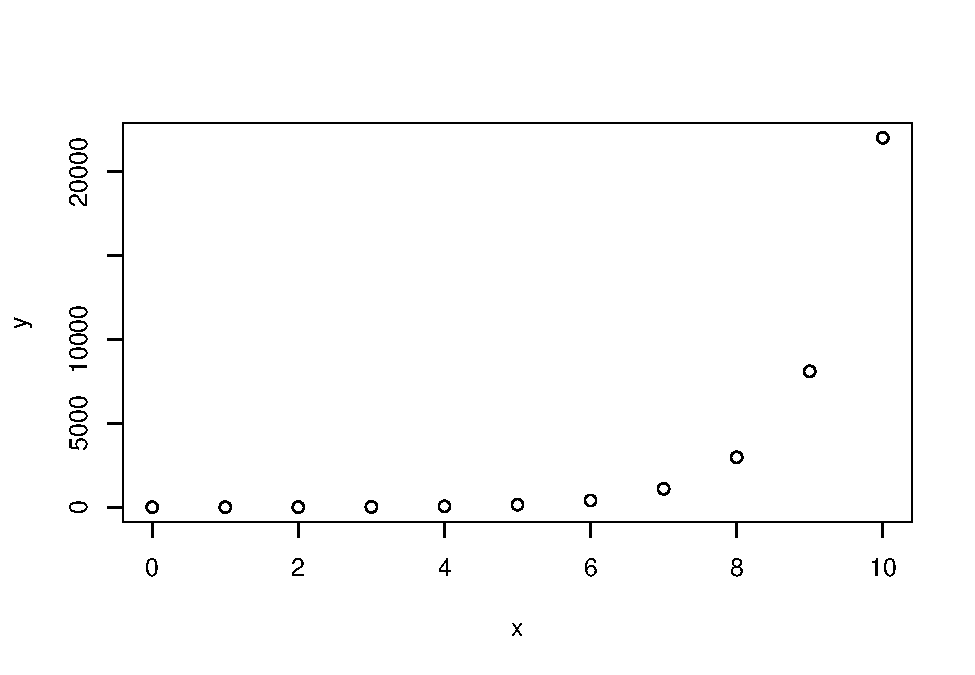
\includegraphics{Toolbox_files/figure-latex/unnamed-chunk-76-1.pdf}

\begin{Shaded}
\begin{Highlighting}[]
\CommentTok{\# toy data}
\NormalTok{x }\OperatorTok{=}\NormalTok{ np.arange(}\DecValTok{11}\NormalTok{)}
\NormalTok{y }\OperatorTok{=}\NormalTok{ np.exp(np.arange(}\DecValTok{11}\NormalTok{))}
\end{Highlighting}
\end{Shaded}

\begin{Shaded}
\begin{Highlighting}[]
\CommentTok{\# default \textquotesingle{}kind\textquotesingle{} is \textquotesingle{}line\textquotesingle{}}
\NormalTok{plt.plot(}
\NormalTok{  x, y,}
\NormalTok{  color }\OperatorTok{=} \StringTok{\textquotesingle{}blue\textquotesingle{}}
  \CommentTok{\# titles are added separately}
\NormalTok{)}\OperatorTok{;}
\NormalTok{plt.title(}\StringTok{\textquotesingle{}Matplotlib line plot\textquotesingle{}}\NormalTok{)}\OperatorTok{;}
\NormalTok{plt.xlabel(}\StringTok{\textquotesingle{}x\textquotesingle{}}\NormalTok{)}\OperatorTok{;}
\NormalTok{plt.ylabel(}\StringTok{\textquotesingle{}$y = e\^{}x$\textquotesingle{}}\NormalTok{)}\OperatorTok{;}
\NormalTok{plt.show()}
\end{Highlighting}
\end{Shaded}

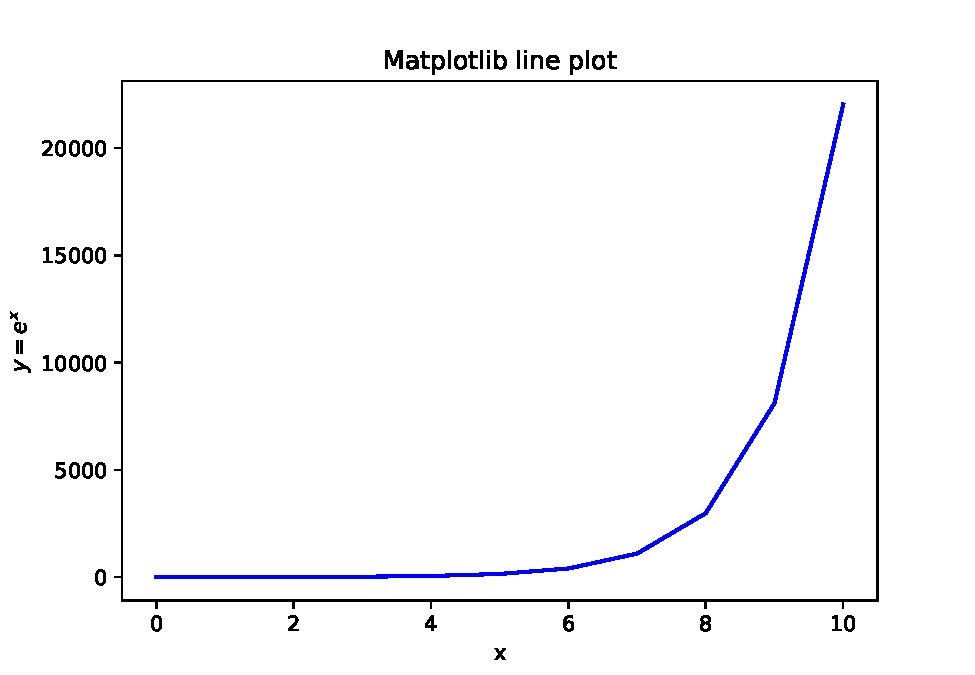
\includegraphics{Toolbox_files/figure-latex/lib-py-1.pdf}

\hypertarget{missing-values-and-duplicates}{%
\chapter{Missing Values and Duplicates}\label{missing-values-and-duplicates}}

\hypertarget{missing-values}{%
\section{Missing Values}\label{missing-values}}

\hypertarget{tidyrdrop_na-vs-pd.dropna-and-pd.notpna}{%
\subsection{\texorpdfstring{\texttt{tidyr::drop\_na()} vs \texttt{pd.dropna()\ and\ pd.notpna()}}{tidyr::drop\_na() vs pd.dropna() and pd.notpna()}}\label{tidyrdrop_na-vs-pd.dropna-and-pd.notpna}}

\begin{longtable}[]{@{}lr@{}}
\toprule
name & age \\
\midrule
\endhead
A & 21 \\
B & NA \\
NA & NA \\
D & 40 \\
\bottomrule
\end{longtable}

\emph{How to drop missing rows or columns?}

tidyr::drop\_na()

pd.dropna() and pd.notna()

\begin{Shaded}
\begin{Highlighting}[]
\CommentTok{\# toy data}
\NormalTok{df }\OtherTok{\textless{}{-}} \FunctionTok{tibble}\NormalTok{(}
  \AttributeTok{name =} \FunctionTok{c}\NormalTok{(}\StringTok{\textquotesingle{}A\textquotesingle{}}\NormalTok{, }\StringTok{\textquotesingle{}B\textquotesingle{}}\NormalTok{,}
           \ConstantTok{NA}\NormalTok{, }\StringTok{\textquotesingle{}D\textquotesingle{}}\NormalTok{),}
  \AttributeTok{age  =}  \FunctionTok{c}\NormalTok{(}\DecValTok{21}\NormalTok{, }\ConstantTok{NA}\NormalTok{,}
           \ConstantTok{NA}\NormalTok{, }\DecValTok{40}\NormalTok{)}
\NormalTok{)}
\NormalTok{df}
\end{Highlighting}
\end{Shaded}

\begin{verbatim}
## # A tibble: 4 x 2
##   name    age
##   <chr> <dbl>
## 1 A        21
## 2 B        NA
## 3 <NA>     NA
## 4 D        40
\end{verbatim}

\begin{Shaded}
\begin{Highlighting}[]
\CommentTok{\# drop missing rows}
\NormalTok{df }\SpecialCharTok{\%\textgreater{}\%} \FunctionTok{drop\_na}\NormalTok{()}
\end{Highlighting}
\end{Shaded}

\begin{verbatim}
## # A tibble: 2 x 2
##   name    age
##   <chr> <dbl>
## 1 A        21
## 2 D        40
\end{verbatim}

\begin{Shaded}
\begin{Highlighting}[]
\CommentTok{\# drop specific variable}
\CommentTok{\# with NaN}
\NormalTok{df }\SpecialCharTok{\%\textgreater{}\%} \FunctionTok{drop\_na}\NormalTok{(name)}
\end{Highlighting}
\end{Shaded}

\begin{verbatim}
## # A tibble: 3 x 2
##   name    age
##   <chr> <dbl>
## 1 A        21
## 2 B        NA
## 3 D        40
\end{verbatim}

\begin{Shaded}
\begin{Highlighting}[]
\CommentTok{\# toy data}
\NormalTok{df }\OperatorTok{=}\NormalTok{ pd.DataFrame(\{}
    \StringTok{\textquotesingle{}name\textquotesingle{}}\NormalTok{: [}
        \StringTok{\textquotesingle{}A\textquotesingle{}}\NormalTok{, }\StringTok{\textquotesingle{}B\textquotesingle{}}\NormalTok{, np.nan, }\StringTok{\textquotesingle{}D\textquotesingle{}}
\NormalTok{    ],}
    \StringTok{\textquotesingle{}age\textquotesingle{}}\NormalTok{: [}
        \DecValTok{21}\NormalTok{, np.nan, np.nan, }\DecValTok{40}
\NormalTok{    ]    }
\NormalTok{\})}
\NormalTok{df}
\end{Highlighting}
\end{Shaded}

\begin{verbatim}
##   name   age
## 0    A  21.0
## 1    B   NaN
## 2  NaN   NaN
## 3    D  40.0
\end{verbatim}

\begin{Shaded}
\begin{Highlighting}[]
\CommentTok{\# drop missing rows}
\NormalTok{df.dropna()}
\end{Highlighting}
\end{Shaded}

\begin{verbatim}
##   name   age
## 0    A  21.0
## 3    D  40.0
\end{verbatim}

\begin{Shaded}
\begin{Highlighting}[]
\CommentTok{\# drop specific variable}
\CommentTok{\# with NaN}
\NormalTok{df[df[}\StringTok{\textquotesingle{}name\textquotesingle{}}\NormalTok{].notna()]}
\end{Highlighting}
\end{Shaded}

\begin{verbatim}
##   name   age
## 0    A  21.0
## 1    B   NaN
## 3    D  40.0
\end{verbatim}

\hypertarget{sql}{%
\chapter{SQL}\label{sql}}

\hypertarget{create-table}{%
\section{Create Table}\label{create-table}}

\begin{Shaded}
\begin{Highlighting}[]
\KeywordTok{DROP} \KeywordTok{TABLE}\NormalTok{ students;}
\CommentTok{{-}{-}{-} create toy table: students}

\KeywordTok{CREATE} \KeywordTok{TABLE}\NormalTok{ students}
\NormalTok{(student\_id }\DataTypeTok{CHAR}\NormalTok{(}\DecValTok{5}\NormalTok{) }\KeywordTok{NOT} \KeywordTok{NULL}\NormalTok{,}
\NormalTok{name }\DataTypeTok{VARCHAR}\NormalTok{(}\DecValTok{10}\NormalTok{),}
\NormalTok{gender }\DataTypeTok{VARCHAR}\NormalTok{(}\DecValTok{6}\NormalTok{),}
\NormalTok{grade }\DataTypeTok{INT}\NormalTok{,}
\KeywordTok{PRIMARY} \KeywordTok{KEY}\NormalTok{ (student\_id));}

\CommentTok{{-}{-} insert data}

\KeywordTok{INSERT} \KeywordTok{INTO}\NormalTok{ students}
\KeywordTok{VALUES} 
\NormalTok{(}\StringTok{\textquotesingle{}SQ001\textquotesingle{}}\NormalTok{, }\StringTok{\textquotesingle{}Barney\textquotesingle{}}\NormalTok{, }\StringTok{\textquotesingle{}Male\textquotesingle{}}\NormalTok{, }\DecValTok{18}\NormalTok{),}
\NormalTok{(}\StringTok{\textquotesingle{}SQ002\textquotesingle{}}\NormalTok{, }\StringTok{\textquotesingle{}Robin\textquotesingle{}}\NormalTok{, }\StringTok{\textquotesingle{}Female\textquotesingle{}}\NormalTok{, }\DecValTok{17}\NormalTok{),}
\NormalTok{(}\StringTok{\textquotesingle{}SQ007\textquotesingle{}}\NormalTok{, }\StringTok{\textquotesingle{}Sheldon\textquotesingle{}}\NormalTok{, }\StringTok{\textquotesingle{}Male\textquotesingle{}}\NormalTok{, }\DecValTok{20}\NormalTok{),}
\NormalTok{(}\StringTok{\textquotesingle{}SQ008\textquotesingle{}}\NormalTok{, }\StringTok{\textquotesingle{}Penny\textquotesingle{}}\NormalTok{, }\StringTok{\textquotesingle{}Female\textquotesingle{}}\NormalTok{, }\DecValTok{13}\NormalTok{);}
\end{Highlighting}
\end{Shaded}


  \bibliography{book.bib,packages.bib}

\end{document}
